%Elsevier-specific stuff
%\documentclass[review]{elsarticle}
\documentclass[5p]{elsarticle}
\usepackage{lineno,hyperref}
\usepackage{tabularx}
\modulolinenumbers[5]
%\bibliographystyle{elsarticle-num}
\bibliographystyle{model2-names.bst}
\biboptions{authoryear}

%Other packages and general latex fields.
\usepackage{url}
\usepackage{color}
\usepackage{graphicx}
\usepackage{epstopdf}

\usepackage{caption}

%%%%%%%%%%%%%%%%%%%%%%%%%%%%%%%%%%%%%%%%%%
\begin{document}
\begin{frontmatter}
\title{gPhoton: Database and Tools for Analysis of Time-Tagged GALEX Photon Events}

% Authors section.
\author[millionconcepts]{Chase Million\corref{chasecorref}}
\cortext[chasecorref]{Corresponding author}

\author[stsci,csc]{Scott W. Fleming}
\author[stsci]{Bernie Shiao}
\author[carnegie]{Mark Seibert}
\author[ucolorado]{Parke Loyd}
\author[appstate]{Michael Tucker}
\author[stsci]{Myron Smith\fnref{myronnewaddress}}
\author[stsci,csc]{Randy Thompson}
\author[stsci]{Richard L. White}
\author[stsci,csc]{Karen Levay}

% Addresses section.
\address[millionconcepts]{Million Concepts LLC, PO Box 119, 141 Mary St, Lemont, PA 16851, USA}
\address[stsci]{Space Telescope Science Institute, 3700 San Martin Dr, Baltimore, MD 21218, USA}
\address[csc]{CSRA, Inc., 3700 San Martin Dr, Baltimore, MD 21218, USA}
\address[carnegie]{The Observatories of the Carnegie Institution of Washington, 813 Santa Barbara Street, Pasadena, CA 91101, USA}
\address[ucolorado]{Department of Astrophysics and Planetary Science, University of Colorado, Boulder CO}
\address[appstate]{Dept. of Physics and Astronomy, Appalachian State University, Boone, NC 28608, USA}
\fntext[myronnewaddress]{Current Address: National Optical Astronomy Observatory, 950 N. Cherry Ave., Tucson, AZ 85719}

% Since \fnref{} in the author page already defines a footnote with a '1' mark, increment the footnote counter now.
\addtocounter{footnote}{1}

\begin{abstract}
gPhoton\footnote{\url{https://github.com/cmillion/gPhoton}} is a new database product and software package that enables analysis of GALEX ultraviolet data at the photon event level. The project's standalone, pure-Python calibration pipeline reproduces the functionality of the original mission pipeline to reduce raw spacecraft data to lists of time-tagged, sky-projected photon events which are then hosted in a publicly available database by the Mikulski Archive at Space Telescope (MAST). This database contains approximately 130 terabytes of data describing approximately 1.1 trillion sky-projected events with a timestamp resolution of five thousandths of a second. A handful of modules serve as a front-end to interact with the database and to generate calibrated light curves and images from the photon-level data at user-defined temporal and spatial scales. The gPhoton software and source code are in active development and publicly available under a permissive license. We describe the motivation, design, and implementation of the calibration pipeline, database, and tools, with emphasis on divergence from prior work as well as challenges created by the large data volume. We summarize the astrometric and photometric performance of gPhoton output relative to the original mission pipeline output and the LDS749B white dwarf standard star. As an example of short time domain science capabilities of gPhoton, we describe new flare observations of the known M dwarf flare star CR Draconis.
\end{abstract}

\end{frontmatter}

%\linenumbers

\section{Introduction}
\subsection{GALEX Overview}
The Galaxy Evolution Explorer \citep{mar2005} was a NASA Small Explorer (SMEX) telescope that surveyed the sky in the ultraviolet over ten years between launch on 28 April 2003 and spacecraft termination on 28 June 2013. The spacecraft, instruments, data and calibration are well described in previous publications \citep{mor2005,mor2007} and the mission'��s online technical documentation.\footnote{\url{http://www.galex.caltech.edu/wiki/Public:Documentation}} We will restrict discussion to topics that are necessary for completeness, have not appeared elsewhere in the literature, or are of particular importance to the gPhoton project.

GALEX carried two micro-channel plate detectors (MCP) with 1.25 degree fields-of-view (FoV), simultaneously exposed via a dichroic. The detectors observed in two broad ultraviolet (UV) bands centered around $1528\,\rm{\AA}$ (Far Ultraviolet or ``FUV'') and $2271\,\rm{\AA}$ (Near Ultraviolet or ``NUV''). The FUV detector failed in May of 2009, but the NUV detector continued to operate until the end of the mission. The spacecraft could observe in either direct imaging or slitless spectroscopic (grism) modes. Observations were conducted while the spacecraft was on the night side of each orbit (an ``eclipse''), which lasted 1500-1800 seconds. To avoid detector burn-in or local gain sag effects caused by depletion of electrons in the multiplier plate, and to smooth over local irregularities in detector response, the telescope did not stare at a fixed location on the sky during an observation but continuously moved the boresight relative to the target position. Several boresight patterns, or ``modes,'' were used over the course of the mission, with consequences for the nature of the corresponding observations and data.

In the most basic ``dither'' mode, the spacecraft boresight would trace out a tight spiral pattern with a radius of $\sim 1'$. Dither mode was used most often for Deep or Medium Imaging Surveys (DIS, MIS) in which a full eclipse was spent observing a single region of the sky. In the All-sky Imaging Survey (AIS) mode, the spacecraft boresight would jump between multiple positions (or ``legs'') on the sky for short integrations of $\sim 100$ seconds each. Between each leg, the detector was set to a non-observing, low voltage state. This resulted in one independent observation (or ``visit'') per leg. A mode called ``petal pattern'' was used to distribute the flux from particularly bright targets across the detector. Petal pattern is in some ways similar to the AIS mode, but with the legs tightly clustered into the approximate area of a single FoV and with the detector remaining in its nominal high-voltage state in between.

On 4 May 2010, an event referred to by the mission team as the ``Coarse Sun Point'' (CSP) anomaly---referring to the safe mode entered by the spacecraft at that time---resulted in image degradation of the NUV detector. The CSP anomaly precipitated severe streaking in the detector's Y-direction, likely due to a failed capacitor. Although the effect was largely corrected through subsequent calibration and onboard adjustments, observations taken between 4 May and 23 June 2010 have substantially worse point spread functions (PSF), and caution should be exercised when comparing observations made before this time range to observations made after to discount bias due to either degraded PSF or uncorrected ``ghost'' photons.\footnote{\url{http://www.galex.caltech.edu/wiki/Public:Documentation/Chapter_8}}

NASA support for the mission ended in February of 2011. At that time, ownership of the spacecraft was transferred to the California Institute of Technology for a phase called the ``Complete the All-sky UV Survey Extension'' (CAUSE), during which operating costs were solicited from individuals or institutions, and spacecraft engineering constraints related to field and source brightness were relaxed, making it possible to observe bright regions of the sky that were off limits during primary mission [CITE]. Spacecraft slew rate limits were also relaxed, permitting a high-coverage ``scan mode'' that swept across several degrees of sky in a single integration. Ownership of the CAUSE-phase data resides with each of the primary investigators, and only a small fraction of it has been made available to the public through MAST at the time of writing, although much of the raw data has been copied to MAST systems. Although the new calibration capabilities of gPhoton may be of particular value in using and interpreting CAUSE data generally and scan mode observations of very bright or dense fields in particular, this paper (and the current gPhoton database) only includes the direct imaging data through the end of the NASA-supported mission, corresponding to General Release 7 (GR7) in the MAST archives. Future work may add gPhoton support for CAUSE phase, scan mode, or spectroscopic data collected throughout the mission. Through GR7, GALEX collected data over 34,389 (direct image) eclipses, which amount to $\sim 18$ TB of raw data and $\sim 14$ TB of reduced image data, covering 76.9\% of the sky in at least one band.

In Section \ref{motivation} we describe the motivation behind constructing the gPhoton database and software suite. In Section \ref{database} we describe the design and content of the $\sim 1.1$ trillion row database hosted at MAST. In Section \ref{softwaretools} we describe the primary modules to use for generating photon lists, light curves and images. In Section \ref{implementation} we discuss implementation challenges we encountered, and our solutions to those problems, some of which may be applicable to other large databases low level scientific data. In Section \ref{calibration} we present tests of the calibration precision by studying the astrometric, relative, and absolute fluxes produced by the software. Finally, in Section \ref{scienceexamples}, we highlight an example science case enabled by gPhoton: stellar flares from CR Draconis.

\section{Motivation}
\label{motivation}
Micro-channel plate (MCP) detectors like those on GALEX are non-integrating detectors---sometimes called ``photon-counting''---that can record position and time information individually for every incident photon (``event''). The GALEX detectors were capable of recording data with a time resolution of five microseconds, though the vast majority of observations were made in a compressed mode at five millisecond resolution. Due primarily to computer storage and processing constraints, calibrated GALEX data was only released and archived by the mission as either per-observation or multi-observation (coadded) image maps with exposure depths on the order of hundreds to thousands of seconds. Although the GALEX mission's data calibration pipeline (hereafter referred to as the ``mission pipeline'') was capable of producing aspect-corrected photon list files (called ``extended'' or ``x-files''), this was rarely done only as part of instrument diagnostics or by special request of members of the scientific community, [CITE Welsh, what else?]. The team produced very little documentation about the detector performance or calibration on timescales shorter than $\sim 100$ seconds.

Advances in data storage and processing capabilities now make archiving, distribution, and analysis of the photon-level data technologically feasible. By the end of the mission, however, the mission pipeline had grown to sufficient complexity and dependence on its software and hardware operating environment that attempts to run it outside of the networked infrastructure upon which it was developed at Caltech proved unsuccessful. We undertook the gPhoton project, in part, to migrate key functionality of the mission pipeline into a stand-alone, open source software base that is robust enough to operating environment to serve as a jumping off point for future researchers to modify or improve the calibration or otherwise build on the legacy of this unique data set. Another major objective was to enable the creation of calibrated light curves and images at user-specified spatial and temporal scales, permitting studies of short time-domain variability in the ultraviolet over a significant fraction of the sky for the first time. The gPhoton project design goals included the following key features:
\begin{itemize}
\item{A stand-alone GALEX calibration pipeline which reproduces the capabilities of the mission pipeline reduce spacecraft data to aspect-corrected photon event data.}
\item{A publicly accessible database containing nearly all photon events from the mission.}
\item{Software that can perform the necessary calibrations (astrometric, photometric, exposure time, etc.), at quality comparable to the original mission pipeline, over visit- and coadd-level timescales.}
\item{An ability to flexibly create images (as a coadd over one or more specified time ranges) or image cubes (as sequences of such coadds).}
\item{An ability to create light curves with a specified time intervals and bins depths.}
\item{Lower the barrier to entry of working with short time domain GALEX data by, e.g., minimizing the number of primary (forward-facing) modules required, wrapping the database queries behind a python interface, creating commonly used output file formats like FITS and comma separated values (CSV), etc.}
\end{itemize}

While the gPhoton project does reproduce much of the core functionality of the mission pipeline, it is not intended as either a full migration or a faithful port of the original mission pipeline. As will be described, some archived output files from the mission pipeline are used where deemed expedient, and the calibration and reduction methodology has been modified in places in service to both computational efficiency and the unique properties and uses of photon-level data.

\section{The Database}
\label{database}
\subsection{Mission Data Products Used By gPhoton}
During the GALEX mission, data were downlinked from the spacecraft and assembled on the ground into monolithic telemetry files (-tlm). The ingest stage of the mission pipeline split these into various types of encoded raw detector event and spacecraft state (-scst) data, which included coarse aspect solutions from the onboard star tracker at one-second resolution, as well as spacecraft housekeeping records. The most important class of encoded raw detector data for gPhoton, containing nominal scientific observations, were the -raw6 files. The -raw6 were decoded with a sequence of bitwise manipulations into lists of raw detector positions ($x$ and $y$) with timestamps for all detector events. These raw positions were further adjusted with ``static'' (detector-space) calibrations for wiggle, walk, nonlinearity and distortion, all described more completely in \citet{mor2007}. For post-CSP data (after eclipse number 37460), the calibration was modified to correct and account for changes to the detector electronics and onboard software. The most substantial of the post-CSP calibration changes was the addition of a processing step to correct for detector streaking caused by the anomaly and correlated strongly to the “YA” value of the raw position data (one of many intermediate raw data values used in derivation of detector event positions).

\subsection{Reduction of the Photon Data}
From the raw photon event (-raw6), refined spacecraft attitude (-asprta), and spacecraft state (-scst) files available at MAST, the celestial coordinates of photon events are calculated and then exported to CSV files. These files contain the time of the photon event, the event positions on the detector, the aspect-corrected positions on the sky (as RA and DEC), and status flags used to track a variety of conditions related to the detector readout. The vast majority of users will only be interested in photon events for which the photon file flag value is equal to zero, indicating nominally processed data.

Only a subset of the photon events from a given eclipse are able to have aspect-corrected positions calculated (most often because only a subset of photon events in an eclipse correspond to an observation, others happen during dead time, slewing, etc.  Therefore, four CSV files are created: one file for each band that contains aspect-corrected photon events, and one file for each band that contains photon events that were not aspect-corrected. The non-aspect-corrected photon events are retained and loaded into a database to be used for estimating dead time corrections (see Section \ref{deadtimedesc} for details). When events cannot be aspect-corrected, their right ascension and declination values are assigned values of \emph{NULL} in the photon list file. For this reason we often refer to uncorrected ``null data'' and nominal or ``non-null data.''

A large fraction of data are not aspect-correctable because they fall in time ranges that are not covered by the refined aspect solutions. Such gaps occur when the detector voltage is ramping up or down between observations or when the slew rate was too high (as between legs of a petal pattern observation) or the stellar field too sparse for the aspect refinement pipeline to obtain a solution. Null events can also arise from cases where events fall outside of the main detector FoV, including data arising from the stims, detector noise, or downlink errors. At present, data that fall within regions of the detector covered by the hotspot mask are also not aspect corrected. Hotspots are regions of the detector known to produce anomalously high signals that are not correlated with the observed scene, often due to hardware flaws or damage. Regions of the detector flagged as containing hotspots should not be used in routine data analysis. Many GALEX hotspots are known to be transient, however, such that the masks often block valid observational data; a planned improvement to the pipeline and database will aspect-correct the masked data and apply the mask in the client side in the same manner as the response correction, at discretion of the user, such that overzealously masked but valid data can be recovered.

\subsection{Database Structure}
For performance optimization purposes, the event-level data is distributed over multiple databases. The non-null (aspect corrected) data are spread across ten different databases organized by celestial declination, with bounding ranges selected to approximately balance the number of rows per database. The ten database tables are further divided into a total of 999 partitions. Each partition is then divided into ``zones'' of $30''$. We make use of the fast zone matching algorithm described in \citet{gra2006} for loading and querying the database. Both the database boundaries and the number of $30''$ zones assigned to each partition were defined so that the databases all have similar sizes. This was accomplished by assuming the total number of photon events in a given eclipse is distributed evenly across that eclipse's footprint. Then, the cross-section of that eclipse's footprint against the zone boundaries is calculated to determine which zones that eclipse overlaps. The number of photons in each zone from this eclipse is estimated based on the cross-sectional area, e.g., if a given eclipse spans two zones, but only 10\% of the eclipse's footprint is in one of the zones, 90\% of its total photon events would be considered to belong to the first zone, and 10\% to the other.

This method of estimating photon events in each zone is imprecise because it assumes photon events are evenly distributed across the eclipse, but it serves as a quick approximation to define the database boundaries and partition assignments by not requiring precise computation of the zone membership for all 1.1 trillion photon events beforehand. The distribution of the ten databases on the sky is shown in Fig. \ref{dbdist}, along with a table summarizing the declination ranges and number of photon events in each database (Table \ref{dbcounts}). Given the possibility that a query could span two or more databases, events are assigned to one and only one database. The majority of normal queries access only a single database, but those that do span more are handled on the server, transparent to both the software and end users.
	Null data which were not aspect corrected reside in a single database that is partitioned and indexed on photon event time. To optimize for common classes of queries, the non-NULL data are indexed in three ways:
\begin{enumerate}
	\item{\emph{zoneID} and photon even \emph{time} - Sky coordinates, a search radius, and a time range are inputs to a number of database cone search functions. The declination and radius are translated into a range of zoneIDs which form the basis for construction of an SQL query.}
	\item{\emph{zoneID}, \emph{RA}, and \emph{Dec} - Often used for sub-queries in the functions described above, and occasionally used in queries where photon even time is not a parameter.}
	\item{Photon even \emph{time} and \emph{flag} value - To optimize queries based on time range alone.}
\end{enumerate}

\begin{figure}
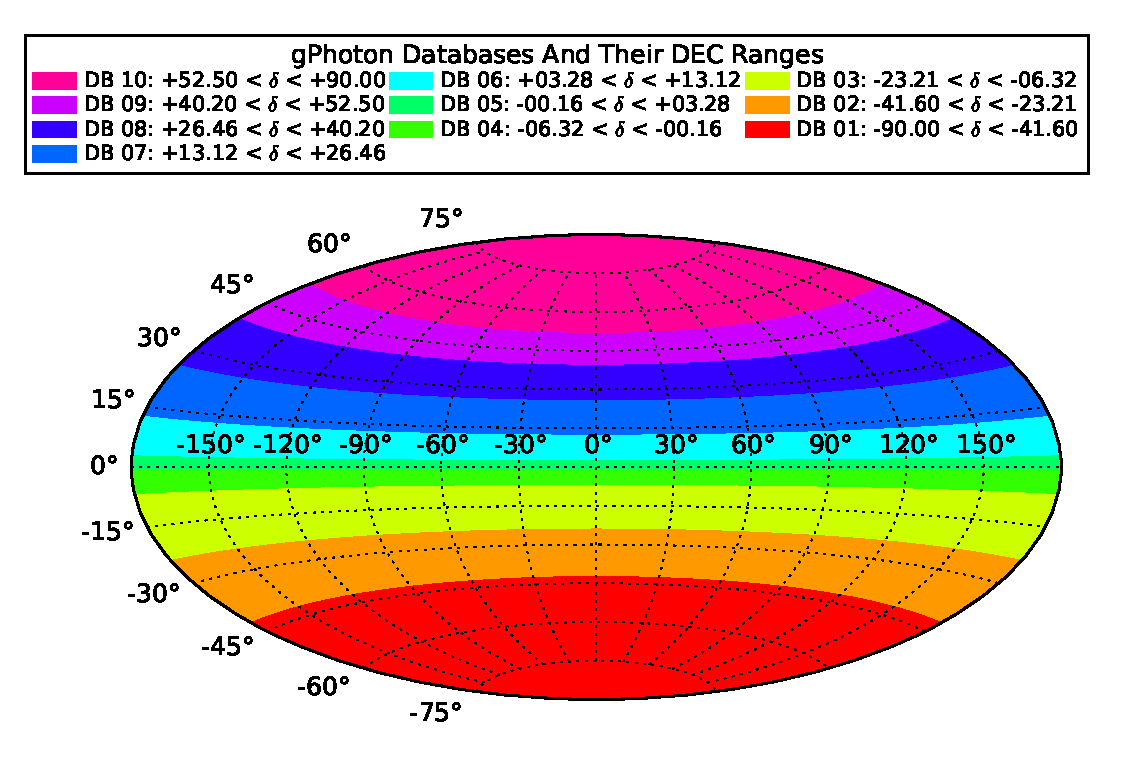
\includegraphics[scale=0.48]{FigDBDist.eps}
\caption{The DEC boundaries of the ten individual databases holding the full corpus of photon data. There are a total of 999 partitions across the ten databases, each with a variable number of $30''$ zones (stripes of DEC).  The number of zones in each partition, and the number of partitions in each database, were assigned so that the size of the ten databases would be roughly equal to each other. \label{dbdist}}
\end{figure}

\begin{table}
\caption{Non-Null Photon Events Per Database\label{dbcounts}}
\begin{tabularx}{.47\textwidth}{lllXX}
\hline\hline
DB & min $\delta$ & max $\delta$ & N\_FUV & N\_NUV\\
   & deg          & deg          & x$10^9$ & x$10^9$\\
\hline
1 & -90.00 & -41.60 &   6.257390699 &  86.634587040\\
2 & -41.60 & -23.21 &   6.381213422 &  86.548536265\\
3 & -23.21 &  -6.32 &   6.581269082 &  86.661438444\\
4 &  -6.32 &  -0.16 &   5.855815141 &  86.824342990\\
5 &  -0.16 &   3.28 &   5.918115466 &  87.675967291\\
6 &   3.28 &  13.12 &   6.431868719 &  86.895361749\\
7 &  13.12 &  26.46 &   6.230197521 &  87.197846131\\
8 &  26.46 &  40.20 &   5.392882518 &  86.855190790\\
9 &  40.20 &  52.50 &   5.394019934 &  86.683794328\\
10 &  52.50 &  90.00 &   6.540819967 & 100.482179843\\
\hline
\end{tabularx}
\end{table}

\section{The Software Tools}
\label{softwaretools}
There are four primary modules included in gPhoton and described in Table \ref{moduledesc}. These utilities are all written in Python and released under a permissive license. With the exception of gPhotonPipe, the tools can be called either from the command line or imported as Python modules. When imported as modules, output is returned in a Python data structure. The command line utilities draw upon a large a large number of supporting functions which will not be described in this paper but are possibly of interest to users who want to perform advanced or specialized analyses with the gPhoton data or even modify the functionality to fit their individual needs. For more information, users are encouraged to consult the documentation available in the software repository, or at the MAST page for the project: \url{https://archive.stsci.edu/prepds/gphoton/}.

While the tools have individual syntaxes to fit their specific functions, a few conventions are standard across all of them. Sky positions are reported as a two-element vectors (right ascension and declination) in J2000 decimal degrees. Time ranges (or ``bins'') are defined as two-element vectors where the first element is the start time and the second element is the end time. The gPhoton project defines timestamps in units of ``GALEX time'' throughout, where $t_{\rm{GALEX}} = t_{\rm{UNIX}} - 315964800$ seconds. To avoid double counting of boundaries, both spatial and temporal ranges are generally taken to be inclusive of the lower value and exclusive of the higher value.

By default, the database tools define an ``effective FoV'' that is 1.1 degrees in diameter, as compared to the full, ``physical FoV'' of the detector at 1.25 degrees. The effective FoV serves as a means to conservatively trim data that lie near the edges of the GALEX MCPs, which regions suffer from uncorrected, transient edge artifacts and poorly understood sensitivity and spatial distortion. The choice of this effective FoV reflects our suggestion that most users simply avoid data collected near the detector edges. Such data \emph{may} be useful, however, to cautious and knowledgeable investigators, so the effective FoV is adjustable from the command line. Critically, the effective FoV (whether using the default or a custom size) does not eliminate problems caused by photometric apertures, annuli, or requested gMap images that extend into (i.e. are clipped by) the boundary of the \emph{effective} FoV. For the most reliable photometry, apertures and image sizes must be clear of the effective FoV boundaries. Apertures and image sizes that extend past the physical FoV should also be avoided. A flag in the gAperture output will alert users to this condition; it is also often visible in gMap movies of the targeted region.

\begin{table}
\begin{tabular}{|p{2cm}|p{6cm}|}
\hline
	{\bf Module} & {\bf Function}\\\hline
	gPhotonPipe & Generates aspect-corrected photon lists from a small set of user supplied input files. The input files are archived products from the original mission pipeline. Output from gPhotonPipe was used to populate the photon event database that the other modules query and, therefore, the majority of researchers will not need this module.\\\hline
	gFind & Provides information on the available raw exposure depths and time ranges for any location on the sky.\\\hline
	gAperture & Generates a light curve (returned as a table of times, calibrated fluxes, and additional parameters) for a given coordinate, time sampling, and aperture size.\\\hline
	gMap & Creates an image (in units of counts and/or calibrated fluxes) and/or image cubes (also in units of counts and/or calibrated fluxes), for a given area of the sky and (optionally) time sampling.\\
\hline
\end{tabular}
\caption{Summary of Primary gPhoton Modules}
\label{moduledesc}
\end{table}

\subsection{gPhotonPipe}
The gPhotonPipe calibration implements a subset of the steps from the original mission pipeline in order to perform detector-level calibration and aspect correction of photon events. The module accepts the raw scientific data file (-raw6), the spacecraft state file (-scst), and one or more refined aspect solution files (-asprta). It returns a ``photon list file'' in CSV format, where each row corresponds to a detector event and records information such as the raw and calibrated detector event positions, sky projected (de-dithered) event positions, and a flag that encodes metadata on the photon event, propagating flags from the aspect solution files and also encoding whether the event falls in a known detector hotspot region. Please see the project documentation for a description of these columns. A flag value of zero at this stage indicates that there were no problems with the calibration of an individual event is the preferred criterion to determine which events should be used by the other tools for later analysis. The photon list files produced by gPhotonPipe are analogous (but not identical) to the extended photon list (-x) files that were occasionally produced (but not archived) by the mission.

Note that all the inputs to the stand-alone calibration pipeline (-raw6, -scst, and -asprta files) are products from the original mission pipeline that are archived at MAST.  By using these archived mission products directly, gPhoton avoids the need to recreate either the ingest or aspect correction stages of the mission pipeline. If an aspect file is not supplied, then gPhotonPipe will attempt to query the MAST database of -asprta data.  Manually specifying the aspect file is possible for researchers who wish to further refine or modify the mission-provided aspect solutions.

\subsection{gFind}
The gFind module allows the user to query the available GALEX exposure depth of a particular target. Given a target position, gFind returns the estimated (raw) exposure depth of available data over the whole mission, separated into time ranges corresponding roughly to discrete observations of the target. Rather than using the visit-based bookkeeping of the mission, which distinguished between observation modes and survey type, gFind uses the photon events themselves. A given position on the sky is considered to be observed if valid data exists in a time range where the position falls within one effective FoV radius of the spacecraft boresight, as defined by the mission-provided refined aspect solution (-asprta). Distinct time ranges are identified based on user-adjustable parameters that define the maximum allowable gap between two events for those data to be considered contiguous (or, in other words, part of the same observation) and the minimum raw exposure depth required for an observation to be considered valid.

\subsection{gAperture}
This module extracts and calibrates event-level data from the database to produce light curves, given user-specified parameters that can include target position, photometric aperture, background annuli sizes, desired integration depth (i.e., bin size), and time range or ranges. Rather than performing photometric measurements on pixelized and integrated images, as the mission pipeline did, gAperture performs aperture photometry by means of cone searches on the sky positions of individual photon events, enabling analysis at the native spatial resolution of the data. Each photon event is weighted by the detector flat value at the spot on the detector on which it occurred, using the mission-produced flats. All events within a given time bin are then weighted by the effective exposure time for the whole detector over that time range. Output from gAperture, which include a very large number of parameters related to the photometric reduction, can be written to CSV-format tables for later analysis. Of note are columns corresponding to bin ranges, effective exposure time, intermediate values such as total number of events within the aperture, calibrated source brightness in counts, physical flux, and AB magnitude units derived with a number of background estimation methods (see below), measurement error, and warning flags coding for a number of conditions that may bias photometric results. Please see the project documentation for a description of gAperture data columns.

\subsection{gMap}
This module creates integrated images and/or image cubes for targeted regions of the sky and specific time ranges, up to and including full depth coadds. Users can request either ``count'' images, which have not been corrected for exposure time or response (often useful for astrometry, diagnostics, or quick-looks), or ``intensity'' images, which are fully calibrated and suitable for photometric analysis. The images produced by gMap are analogous to the imaging data products produced by the mission pipeline, but with additional flexibility via user-adjustable parameters (e.g. dimensions, depth, edge trimming). If given a sequence of time ranges or a bin size, gMap will also produce ``count'' and/or ``intensity'' image cubes (i.e. movies), which the original mission pipeline could not produce at full spatial resolution. All images are written in the Flexible Image Transport System (FITS) format that include headers populated using the World Coordinate System (WCS) standard.  As with relative response correction in gAperture, rather than generating a relative response map, the individual events are simply weighted by the flat value assigned to the detector regions on which they fell. In the current release, the exposure depth at the center of field is applied evenly across the whole image. This is not a good approximation in a large number of cases, particularly when the diameter of the image is not a small fraction of the diameter of the detector FOV; a spatially aware exposure time correction is planned for a future software build.

\section{Calibration Tests}
\label{calibration}
We performed both relative and absolute tests of gAperture performance, comparing gPhoton output to that of the mission pipeline (as recorded in the MCAT) and to white dwarf calibration standard stars LDS749B. In all cases of relative comparisons against the MCAT, the catalog source center positions and observation time ranges were used as inputs to gAperture on a per-visit basis. Except where otherwise noted, a circular photometric aperture of 6'' was used, equivalent to the MCAT \emph{APER4} column, and the gAperture background annulus was defined to extend from 30'' to 90''. When appropriate, source brightnesses (from both gAperture and MCAT) were aperture corrected using the table defined in Figure 4 of \cite{mor2007}. Also except where noted, ``random'' source positions were determined by using a random number generator to draw right ascension and declination positions on the sky as the center positions of a 0.1 degree cone searches of the MCAT for all sources between 14 and 24 AB Magnitude an with less than 5000 seconds of total raw exposure coverage (to avoid biasing the analysis with a small number of sources from a handful of very deep fields).

Where blue curves are overplotted on histograms, these represent Gaussian Kernel Density Estimates (KDE) with bandwidths chosen by brute force cross-validation. The peak of the KDE is reported as the peak of the distribution of data along with a single number denoting the upper and lower extents of an envelope within which 90\% of the data reside. To give a sense of the skew of the distribution, we also report the median value of all data along the same axis. For ease of interpretation, it will be useful to note that, under a linear approximation near zero, a difference of magnitudes can be interpreted as a percent difference.

The source data for all of the calibration plots, the gPhoton commands used to generate the source data and the Python scripts used to create the graphics and results are included as online supplements to this paper. We encourage researchers to use these as starting points to generate error analyses appropriate to their specific projects.

\subsection{Astrometric Reproducibility}
In figures \ref{nuvastrometry} and \ref{fuvastrometry}, we compare the MCAT source center positions to the centers-of-brightness (that is to say, the mean photon position) within a 6'' aperture. The relative astrometry is very good, showing highly symmetrical distributions with strong peaks at zero (indicating no difference in source position) in both Right Ascension (RA) and Declination (Dec) for both bands. The slightly larger dispersion in the distribution for FUV is attributable to lower signal to noise for sources in this band overall. One possible cause of divergence in astrometry between gAperture and the MCAT is that the center of brightness was calculated by the mission pipeline on an image with 1.5'' pixels, necessarily requiring interpolation, whereas gAperture directly samples the detector positions of the incident photons.

\begin{figure}
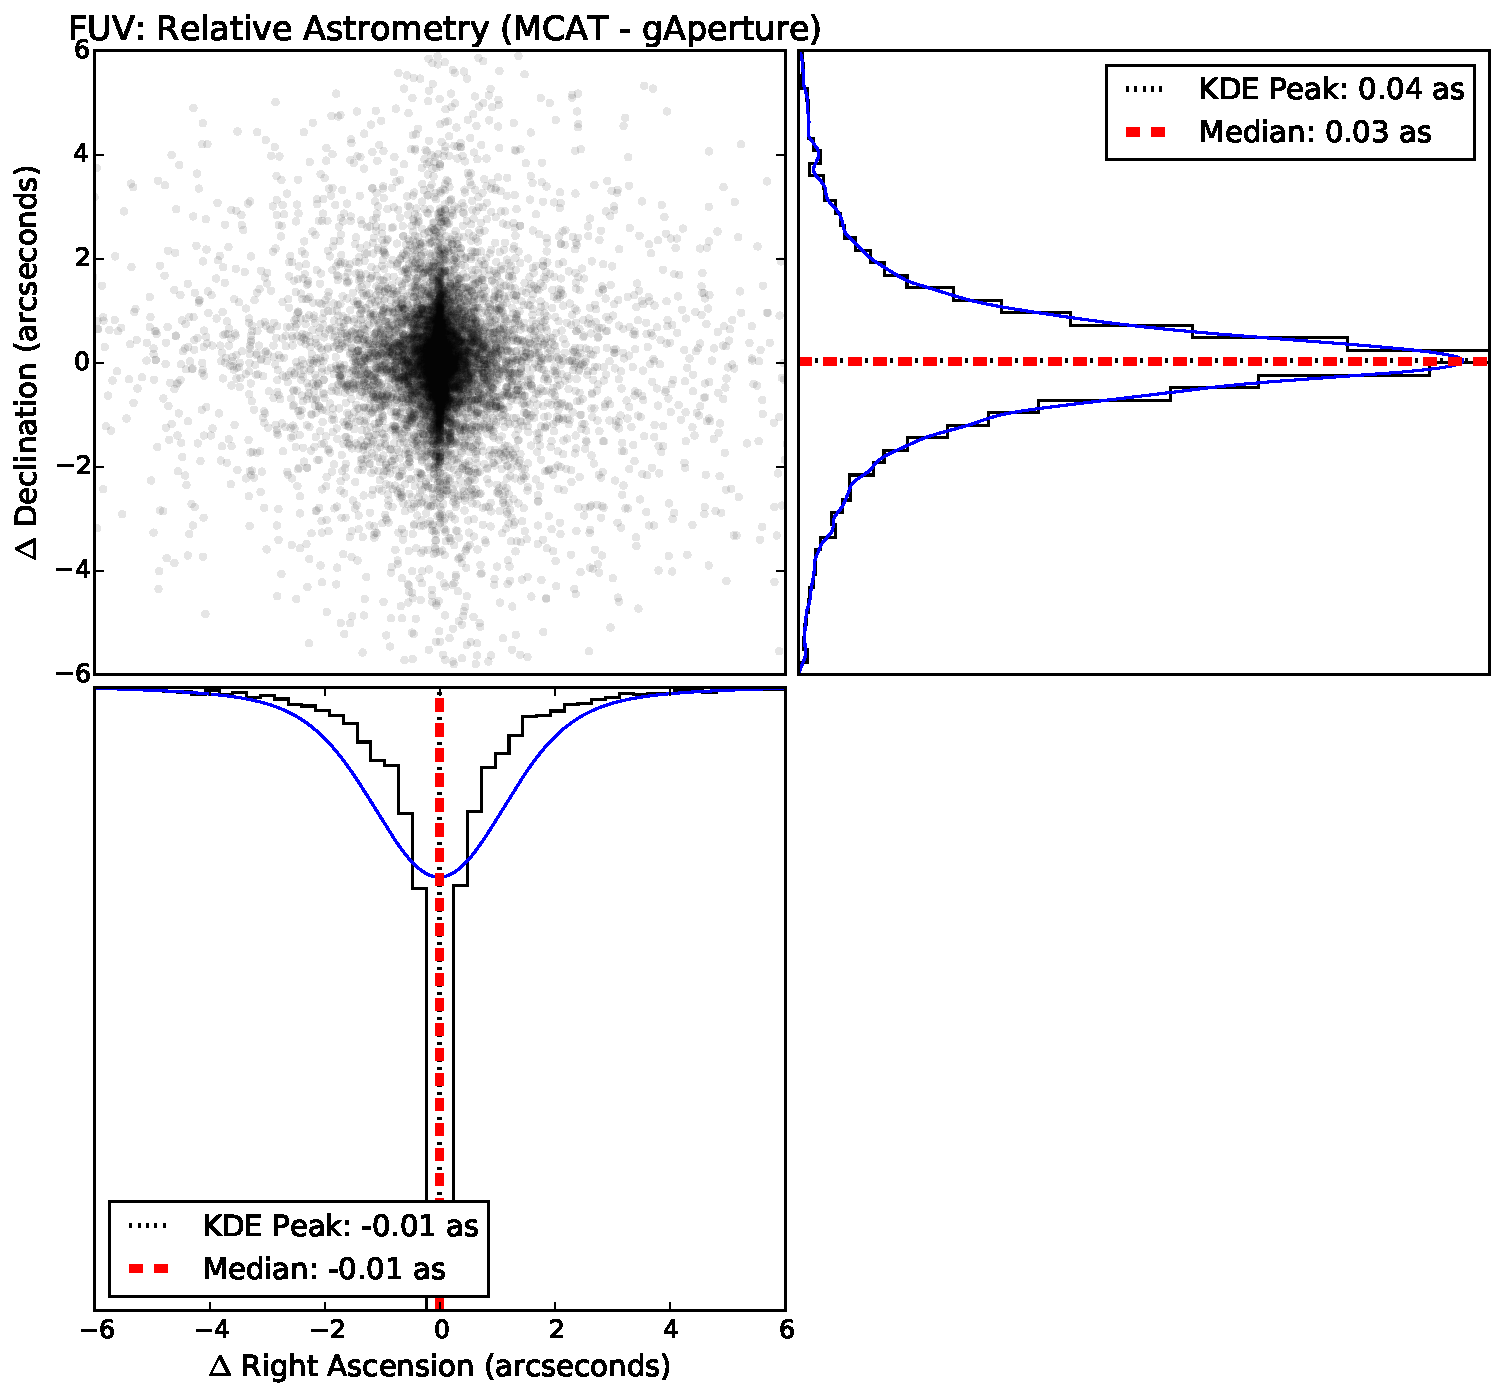
\includegraphics[scale=0.35]{RelAstrometryFUV.pdf}
\caption{Relative offsets between mission catalog (MCAT) source positions and gAperture centers-of-brightness, in the FUV band, within photometric apertures with 6 arcsecond radii.
\label{fuvastrometry}}
\end{figure}

\begin{figure}
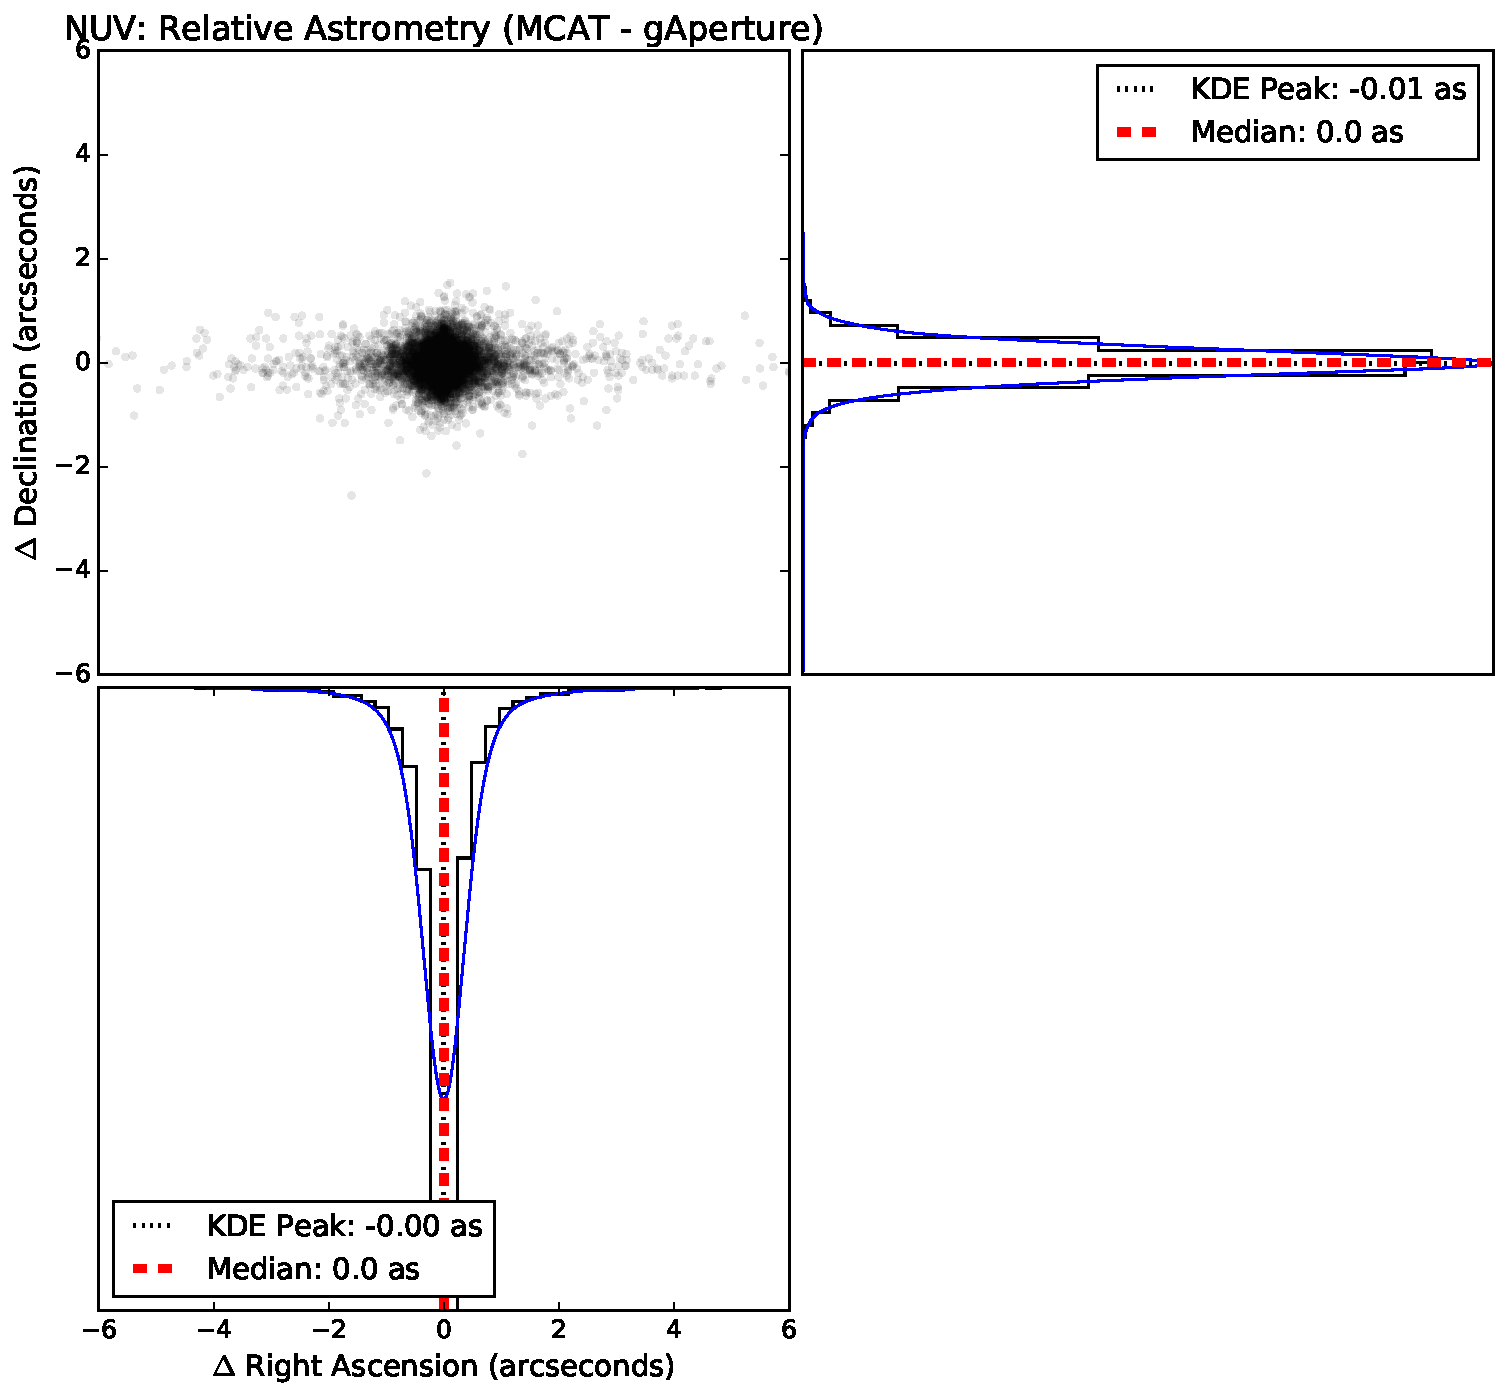
\includegraphics[scale=0.35]{RelAstrometryNUV.pdf}
\caption{Relative offsets between mission catalog (MCAT) source positions and gAperture centers-of-brightness, in the NUV band, within photometric apertures with 6 arcsecond radii.
\label{nuvastrometry}}
\end{figure}

\subsection{Background Correction}
At present, gAperture implements two methods to estimate the contribution of background to measured source brightness. The first simply uses the background values reported in the \emph{NUV\_skybg} and \emph{FUV\_skybg} columns of the mission-produced MCAT catalog on a per-visit basis. That is, gAperture performs a search of the MCAT for the nearest source to the requested sky position and at the requested time. The mission-produced background flux per area recorded for this source is scaled it to the aperture and subtracted from the source flux measured by gAperture. Very broadly, the background estimation procedure in the mission pipeline\footnote{\url{http://www.galex.caltech.edu/DATA/gr1_docs/Background_determination_and_source_extraction_for_GALEX_data.pdf}} used an iterative ``sigma-clipping'' method, modified to make use of the full Poisson distribution, to construct diffuse background maps from sky intensity maps. Measurements of the sky background were then made from these maps by the source extraction stage of the pipeline that ultimately produced the MCAT values.

The second background method implemented by gAperture is a simple annulus estimate where the surface flux within a user-defined annulus surrounding the extraction aperture is scaled to the area of the aperture and subtracted from the source flux. The annulus background method can produces biased results in cases where it captures light from relatively bright nearby sources, although that effect can often be mitigated by carefully defining the annulus to avoid such contamination. As discussed extensively in \ref{deadtimedesc} below, the diffuse sky background in GALEX observations can vary quite substantially over the course of an eclipse due to changes in the ambient terrestrial airglow as the spacecraft traveled from limb to limb. When constructing light curves with the intention of looking for short time domain variability, the annulus background method will correct for this variable diffuse background. Also, under the assumption that any contaminating sources are \emph{not} variable, an overestimate of background flux will not change \emph{relative} photometry of the target source over time (although it has consequences for the error analysis, as will be discussed in \ref{fluxuncert}). We recommend that the annulus background method be used for studies of variability over time scales shorter than a GALEX eclipse.

A comparison of surface fluxes produced by the two methods (Fig. \ref{bgrelphot} demonstrates that the annulus background estimation method consistently overestimates the background surface flux in both bands as compared to the MCAT, as expected by the possibility of unmasked background sources. The effect is much more pronounced in NUV (at $\sim 16\%$ difference on average) than FUV ($\sim 1\%$), probably because there are simply fewer total GALEX-resolvable FUV sources in the sky. It's worth emphasizing again that the analysis in this calibration test naively used the same annuli for all sources; the relative difference between the methods could be mitigated in many cases by carefully (i.e. manually) defining the extents of the annuli. We suggest that researchers routinely check the MCAT as well as a gMap-produced images of the targeted regions for nearby sources that might bias  gAperture photometry.

During development, we also tested two variations of the annulus method that might have mitigated the presence of stars in or near the background annulus. The first method, which we called ``swiss cheese,'' mimicked that applied by Morrissey in the analysis of the GALEX standard star LDS749B \citep{mor2007}: nearby bright stars from the MCAT out to several $\sigma$ (assuming two-dimensional Gaussian profiles of the sources) were masked out by excluding those data and sky regions from subsequent calculations. The second method was an attempt at a direct port of the ``sigma-clipping'' algorithm used by the mission pipeline. Both of these methods were abandoned because they were computationally complex, sensitive to somewhat arbitrary input parameters, and produced poor agreement with catalog fluxes. We may revisit these and other methods for background estimation in future work.

\subsection{Relative Flux Precision}
As a test of the relative photometric precision from gPhoton, we plot the difference between the MCAT magnitude and gAperture magnitude against the MCAT magnitude for 7692 and 20213 randomly selected MCAT sources in FUV and NUV respectively. Fig. \ref{fuvrelphot} and Fig. \ref{nuvrelphot} use the background estimated from the gAperture background annulus, while Fig. \ref{fuvrelphotmcat} and Fig. \ref{nuvrelphotmcat} use the per-visit MCAT background. To a first-order approximation, Although both methods show good agreement on average, with higher dispersion for lower source brightnesses, the MCAT background method has a more symmetric distribution overall.

\begin{figure*}
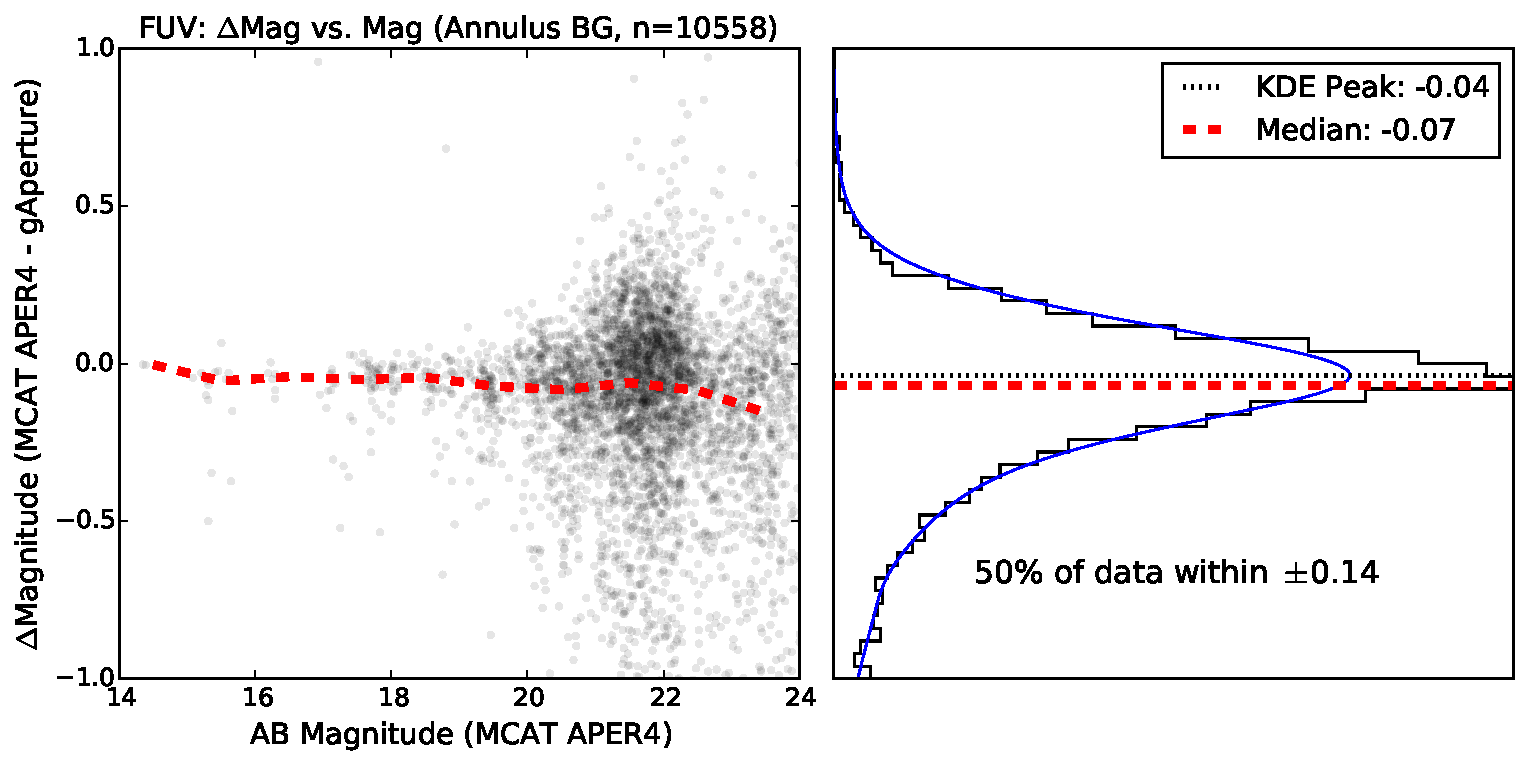
\includegraphics[scale=0.7]{FigRelPhotFUV-annulus_bg.pdf}
\caption{Comparison between MCAT and gPhoton FUV fluxes, using backgrounds estimated from unmasked annuli, for 7692 randomly selected MCAT sources. The dashed line denotes the median difference in half magnitude bins. 
\label{fuvrelphot}}
\end{figure*}

\begin{figure*}
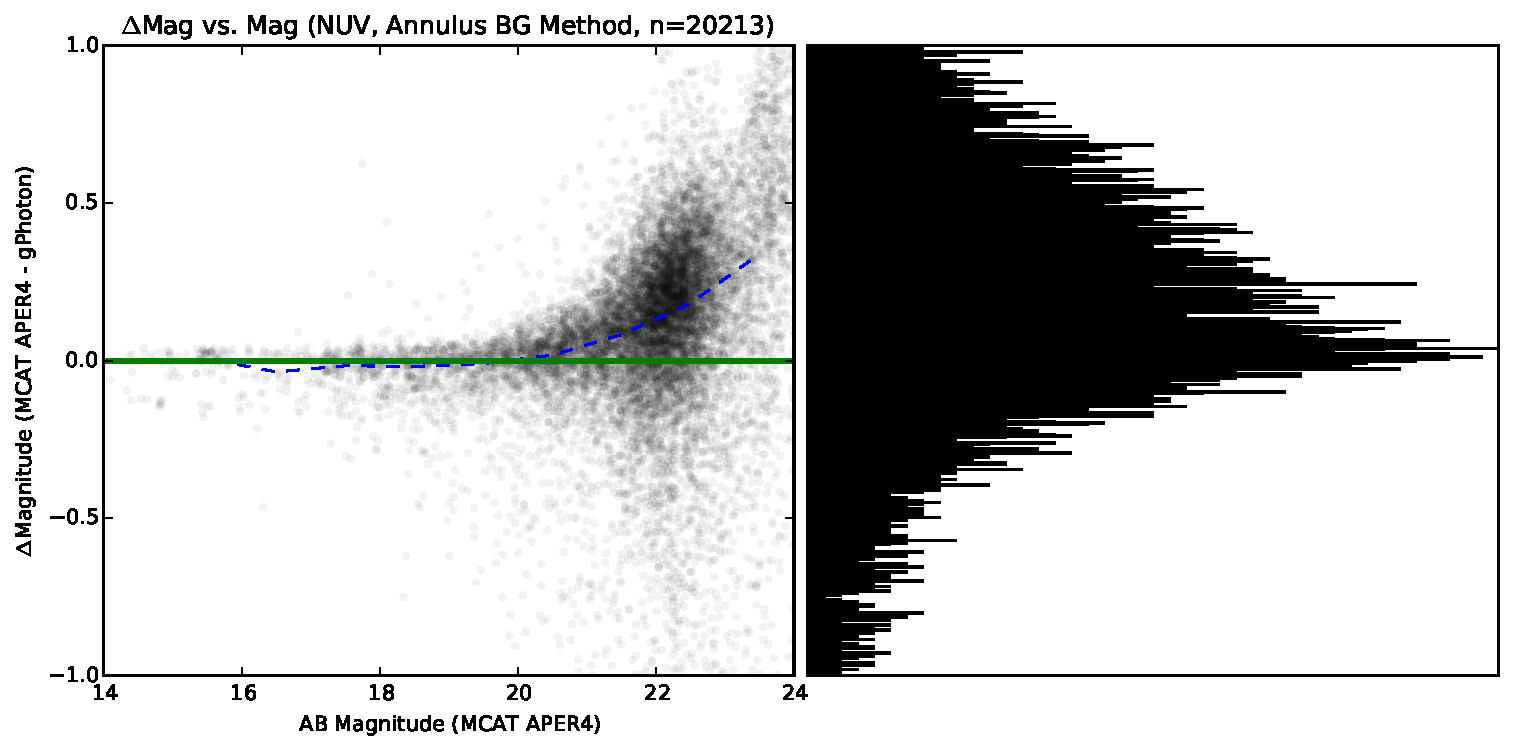
\includegraphics[scale=0.7]{FigRelPhotNUV-annulus_bg.pdf}
\caption{Comparison between MCAT and gPhoton NUV fluxes, using backgrounds estimated from unmasked annuli, for 20213 randomly selected MCAT sources. The dashed line denotes the median difference in half magnitude bins.
\label{nuvrelphot}}
\end{figure*}

\begin{figure*}
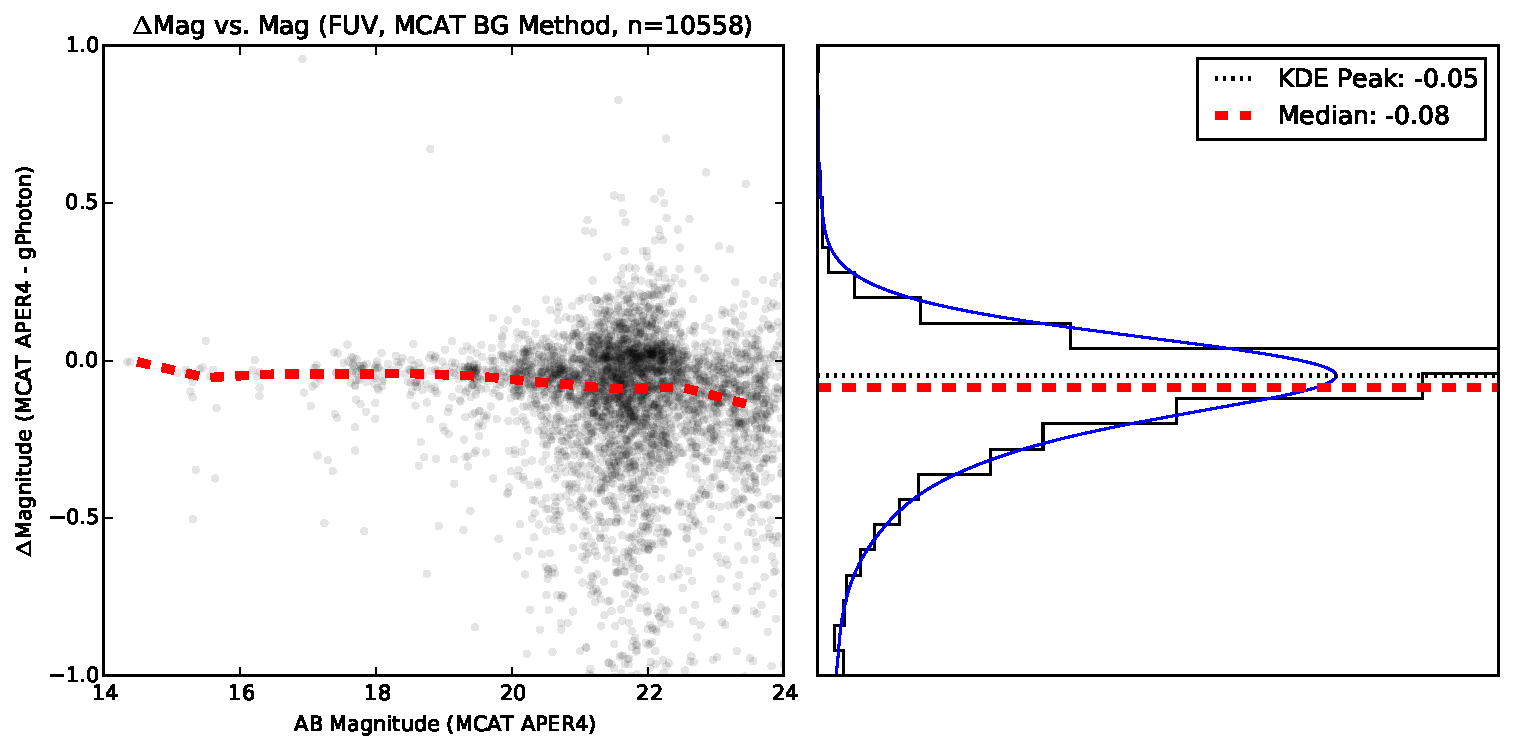
\includegraphics[scale=0.7]{FigRelPhotFUV-mcat_bg.pdf}
\caption{omparison between MCAT and gPhoton FUV fluxes, using background estimates drawn from the visit-level MCAT, for 7692 randomly selected MCAT sources. The dashed line denotes the median difference in half magnitude bins.
\label{fuvrelphotmcat}}
\end{figure*}

\begin{figure*}
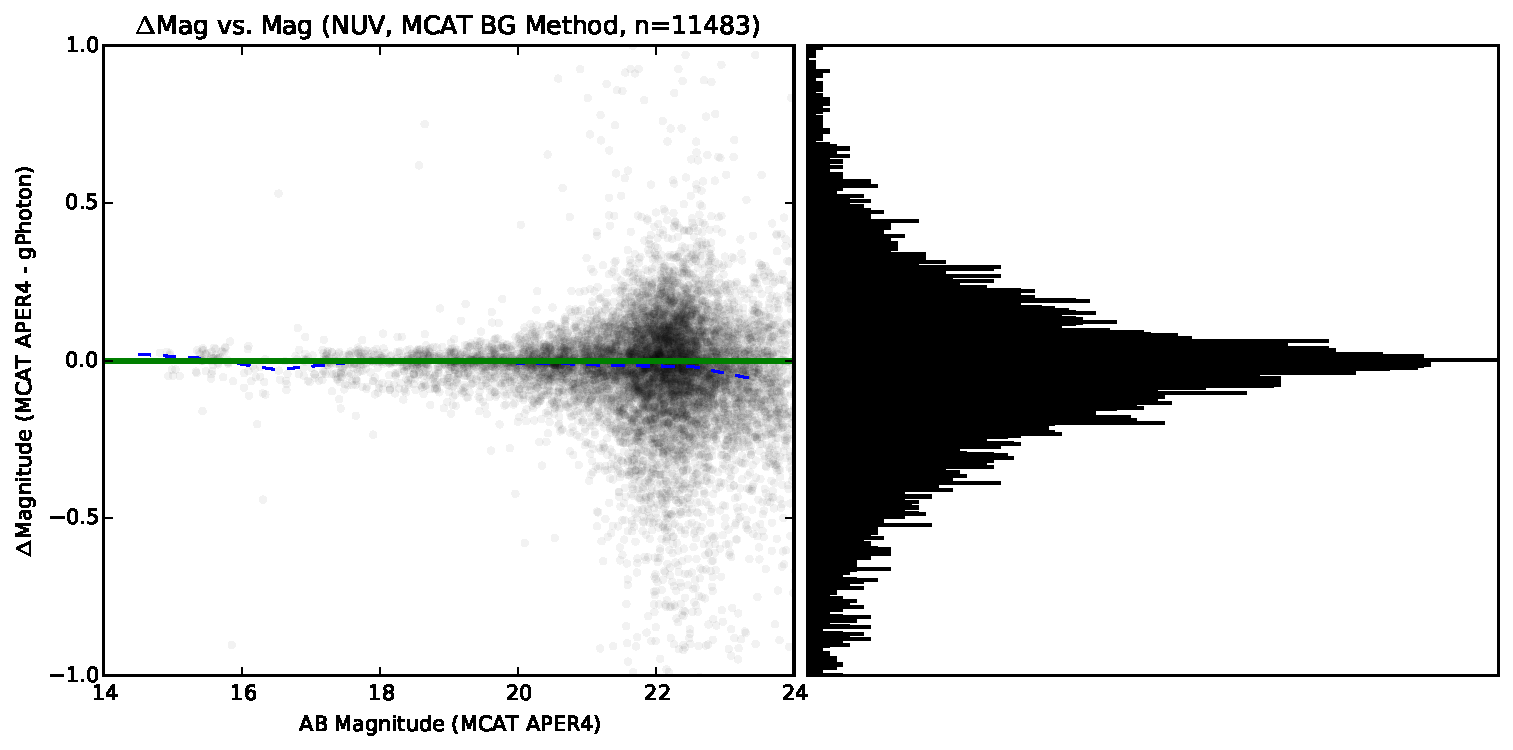
\includegraphics[scale=0.7]{FigRelPhotNUV-mcat_bg.pdf}
\caption{Comparison between MCAT and gPhoton NUV fluxes, using background estimates drawn from the visit-level MCAT, for 20213 randomly selected MCAT sources. The dashed line denotes the median difference in half magnitude bins.
\label{nuvrelphotmcat}}
\end{figure*}

\begin{figure}
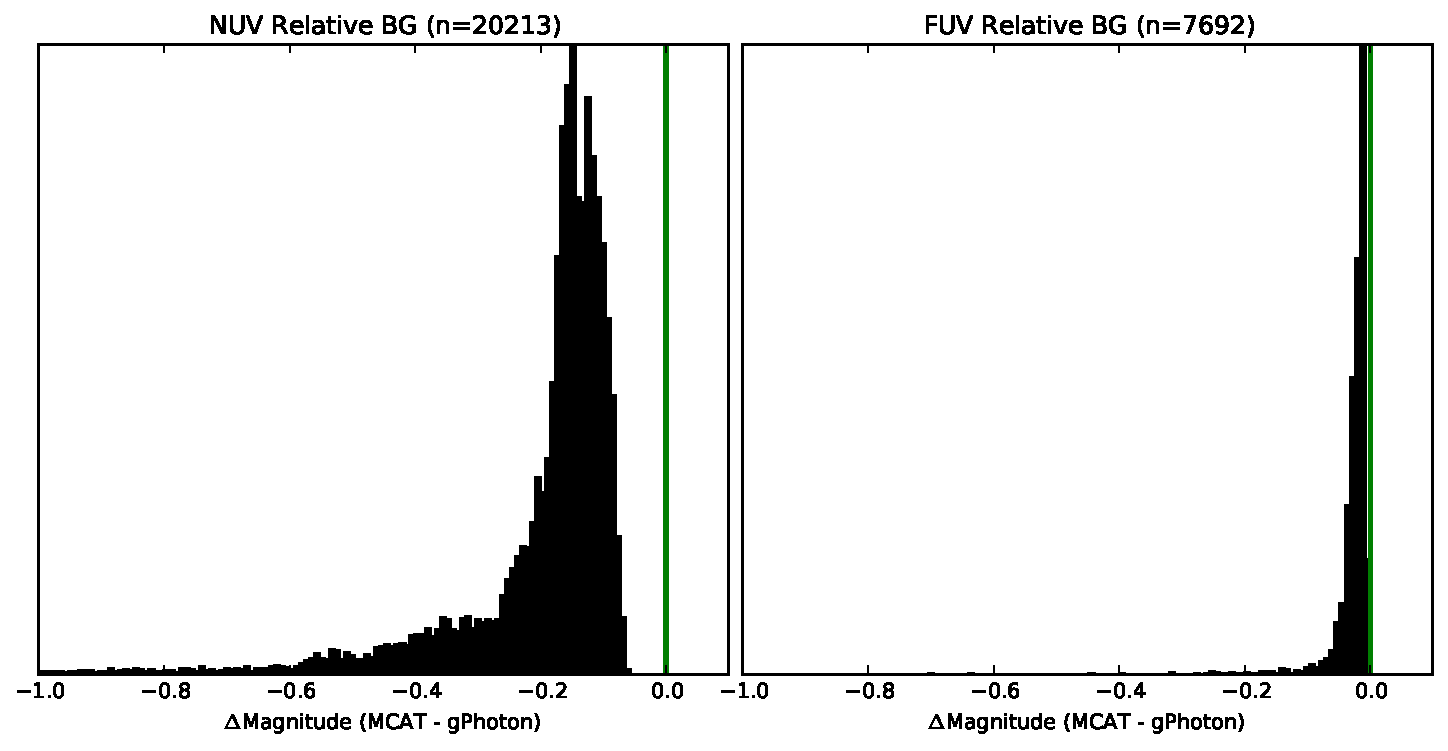
\includegraphics[scale=0.35]{BG_dMag.pdf}
\caption{Effective surface brightness within a 6 arcsecond aperture for the gAperture unmasked annulus method of background estimation as compared to estimates drawn from visit-level MCAT.
\label{bgrelphot}}
\end{figure}

\subsection{Absolute Flux Precision}
As described in \citet{mor2007}, the GALEX mission used the white dwarf LDS749b as the primary calibration reference source. As a test of the \emph{absolute} photometric accuracy of gPhoton, we have compared gAperture photometry for both of these stars to the nominal reference magnitudes in both bands.

[CITE] A total of \{259909, 595672\} seconds of exposure depth in the FUV and NUV bands, respectively, were made on this source. We use gAperture to compute magnitudes for all of these observations in both bands and compare them against the standard magnitudes used by GALEX (Figs. \ref{ldsabsphotfuv},\ref{ldsabsphotnuv}). We measure fluxes separated into visit levels to match the exposure times in the MCAT.

All visit-level MCAT detections within 0.001 degrees of the nominal source position for each source were used as the basis to generate gAperture photometry over matching time ranges and at matching sky positions. We used a photometric aperture with a 0.025 degree (90 arcsecond) radius and an annulus extending from 0.025 to 0.05 degrees. The particularly large aperture corresponds to the largest custom aperture used by \cite{mor2007} to enclose the maximum amount of flux, and the substantial annulus is only contaminated by a small number of relatively faint (>20 AB Mag) stars.

\begin{figure}
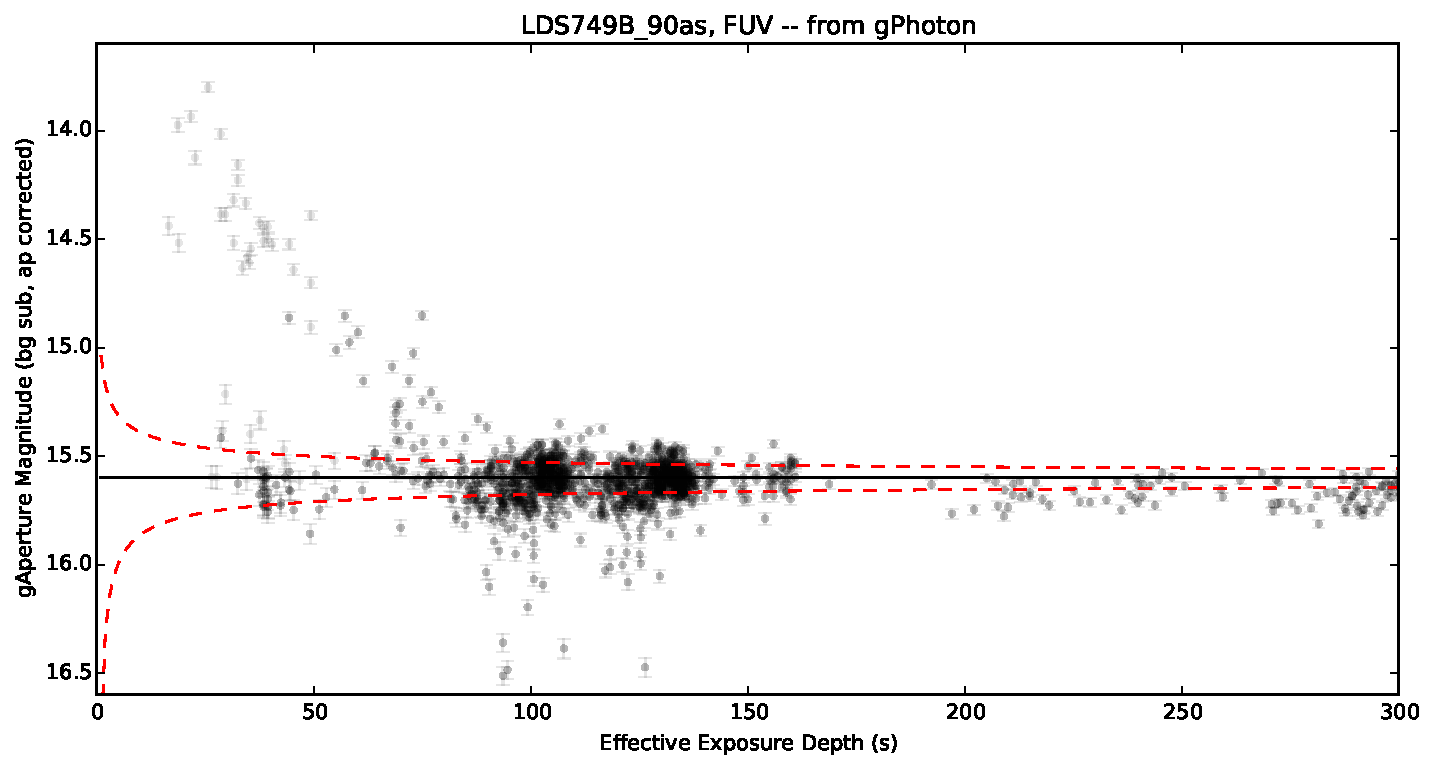
\includegraphics[scale=0.5]{LDS749B_90as_ABMag_FUV.pdf}
\caption{Comparison of gPhoton FUV fluxes for LDS749B to the catalog reference value of 15.57 AB Mag (solid line) as a function of exposure depth. The aperture had a radius of 90'' and backgrounds were estimated with an unmasked annulus extending from 90'' to 180''. The dashed lines denote ideal 3$\sigma$ scatter as predicted from counting statistics. The error bars on the points denote 1$\sigma$.
\label{ldsabsphotfuv}}
\end{figure}

\begin{figure}
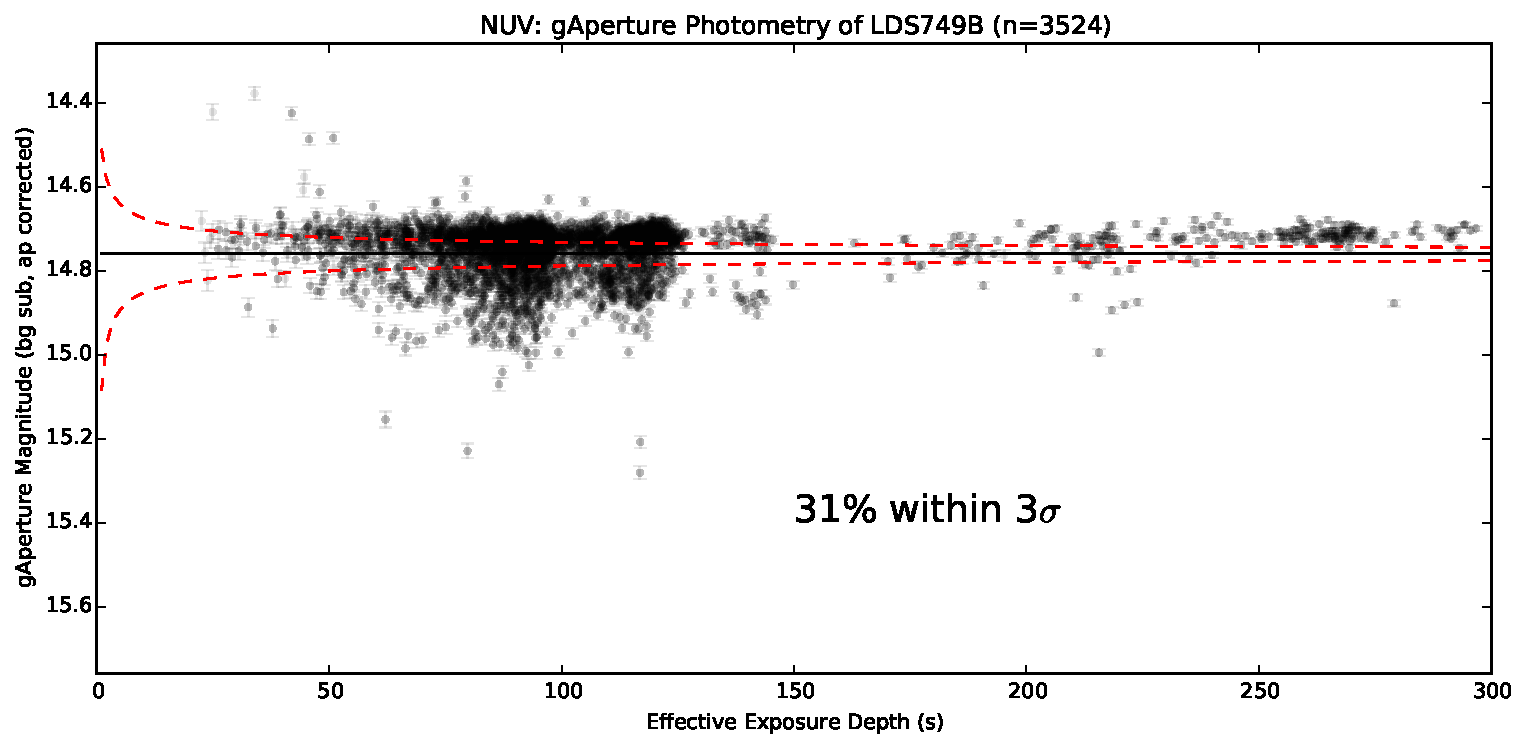
\includegraphics[scale=0.5]{LDS749B_90as_ABMag_NUV.pdf}
\caption{Comparison of gPhoton NUV fluxes for LDS749B to the catalog reference value of 14.71 AB Mag (solid line) as a function of exposure depth. The aperture had a radius of 90'' and backgrounds were estimated with an unmasked annulus extending from 90'' to 180''. The dashed lines denote ideal 3$\sigma$ scatter as predicted from counting statistics. The error bars on the points denote 1$\sigma$.
\label{ldsabsphotnuv}}
\end{figure}

\begin{figure}
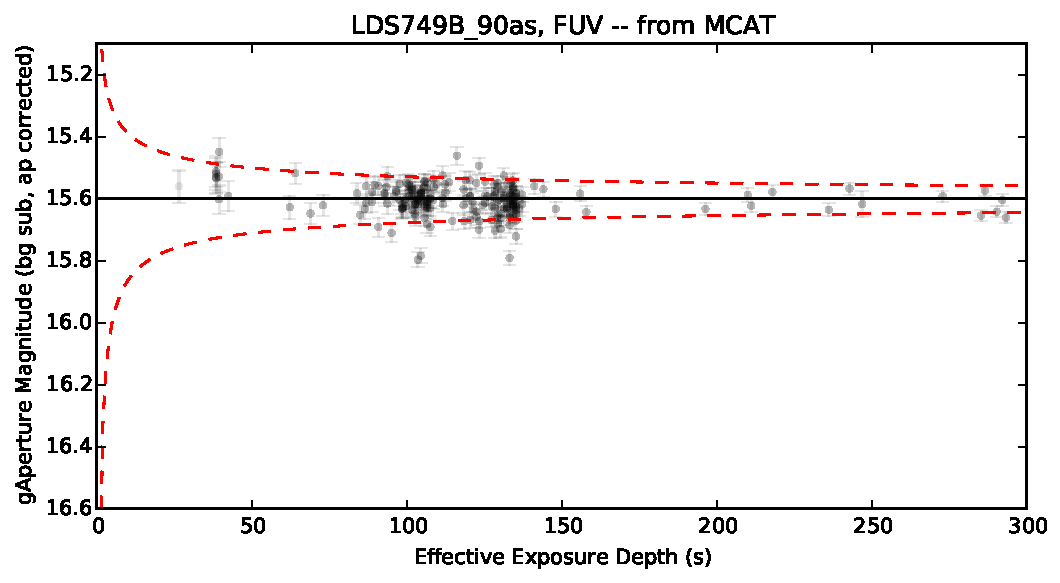
\includegraphics[scale=0.5]{LDS749B_90as_ABMag_FUV_MCAT.pdf}
\caption{Comparison of gPhoton FUV fluxes for LDS749B to the catalog reference value of 15.57 AB Mag (solid line) as a function of exposure depth. The aperture had a radius of 90'' and backgrounds estimates were drawn from the visit-level MCAT. The dashed lines denote ideal 3$\sigma$ scatter as predicted from counting statistics. The error bars on the points denote 1$\sigma$.
\label{ldsabsphotfuvmcat}}
\end{figure}

\begin{figure}
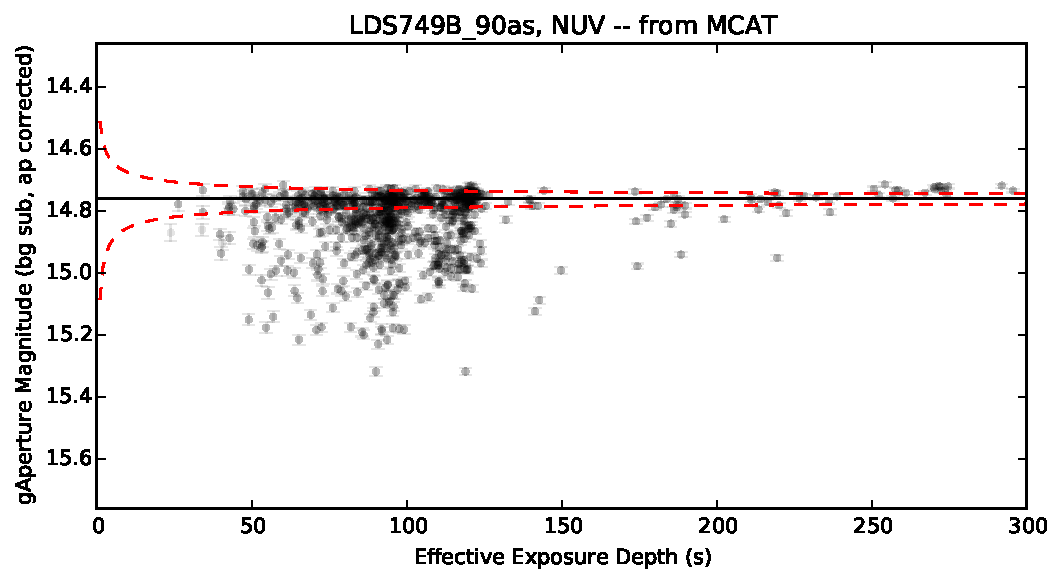
\includegraphics[scale=0.5]{LDS749B_90as_ABMag_NUV_MCAT.pdf}
\caption{Comparison of gPhoton NUV fluxes for LDS749B to the catalog reference value of 14.71 AB Mag (solid line) as a function of exposure depth. The aperture had a radius of 90'' and background estimates drawn from the visit-level MCAT. The dashed lines denote ideal 3$\sigma$ scatter as predicted from counting statistics. The error bars on the points denote 1$\sigma$.
\label{ldsabsphotnuvmcat}}
\end{figure}

\section{Implementation Notes}
\label{implementation}

\subsection{Effective Exposure Time}
\label{effexptime}
The GALEX ``effective exposure time'' is defined as the raw exposure time, minus the amount of time considered ``shuttered,'' scaled by the global dead time ratio.

\[t_e=(t_r-s)*d\]

The raw exposure time (tr) is simply the observation end time minus the observation start time, or what most astronomers would normally think of as the observation exposure time. Any time period of 0.05 seconds or longer during which no valid data was recorded by the detector (i.e. with calibration flag of zero) is considered \emph{shuttered}; the sum of time over such periods during the observation is the shutter correction (s). These might be periods during which the spacecraft was not actually observing the requested region of sky, but can also include data dropouts or periods during which a valid aspect solution is not available for any number of reasons, including being near the beginning or end of an observation or a failure of the aspect refinement stage of the mission pipeline. The global deadtime ratio (d)---described more completely in the following section---is the estimated fraction of time during which incident events were \emph{missed} due to detector readout. For aperture photometry, the effective exposure is computed at the requested sky position, and then applied uniformly across all events in both the aperture and background annulus. This approximation is more efficient than calculating the exposure across the whole region and fails only when the annulus or background contains a masked part of the detector (e.g. hotspots as described below) or crosses the edge of the effective FoV.

\subsection{Exposure Dead Time Correction}
\label{deadtimedesc}
Microchannel plates are subject to a global exposure ``dead time'' effect caused by the inability of the detector to process more than one event at a time. That is, while a single event is being recorded by the detector electronics, other incident events go undetected. The effect scales as a function of total global detector count rates, or the totality of all events (both NULL and non-NULL) recorded by the detector: as global count rates go up, the fraction of exposure lost to dead time likewise increases, and is linear up to approximately 109 counts per second (cps) in FUV and 311 cps in NUV---\citep[demarcating 10\% rolloffs in response,][]{mor2007}. Other MCP instruments have used this global count rate relationship as a means to estimate the dead time correction factor {\color{red}CITE}. The GALEX detectors, however, were equipped with four built-in electrical pulsers (``stims'') located off the main detection window that produced a known rate of events (nominally 79 cps between all four). The mission pipeline estimated a correction by observing that the ratio of the measured stim count rate to the nominal stim count rate should be roughly equivalent to the ratio of the effective exposure time to the raw exposure time. While this "deadtime ratio" varies quite a bit between and even within observations, a typical value is around 0.8 (indicating that 20\% of exposure time is ``lost'' to dead time).

While the stim rate technique used by the mission works well over long integrations, it introduces unacceptable error in exposure time estimates over shorter integrations. At the typical deadtime value of 0.8 noted above, the detected stim count rate (across all four stims) would be approximately 63.2 cps (80\% of the nominal rate of 79 cps). For an AIS-depth integration of 100 seconds, over which $\sim 6320$ stim events would be detected, the 1 {\color{red}sigma} counting error in the stim measurement would be $\sim 79.5$ counts, corresponding to 1.25\% error in the estimated exposure time. This amount of uncertainty is small as compared to other sources in the imaging chain, and, indeed, was not even propagated by the mission pipeline. But with a raw exposure of \emph{just one second}---a commonly desirable light curve bin depth for gAperture---the 1 {\color{red}sigma} counting error would $\sim 7.95$ counts or 12.6\%; with the stim method of estimating dead time, it would not be unusual to mis-estimate the effective exposure over short time intervals, and therefore source brightness, by as much as a third.

gPhoton mitigates this by using the linear relationship between global count rate and dead time, which holds for the majority of global count rates observed by GALEX up through GR6/7, to produce an \emph{empirical} exposure time correction as a function of global count rate. GALEX has typical global count rates of 10,000 cps or more, making the 1$\sigma$ error due to counting statistics truly negligible even for short integrations. The GALEX team did produce such an empirical dead time formula but, while the result was recorded, the actual methodology was not, making it impossible to verify. We know that the behavior of the detectors was deemed in that analysis to be sufficiently similar that an identical model fit was used to describe both of them, and the nominal / commanded stim rate was assumed to be \emph{true} (i.e. the stim rate at ``zero'' global counts was fixed to 79 cps). For completeness and consistency, we have redone this empirical deadtime analysis without those two assumptions.

\begin{figure}
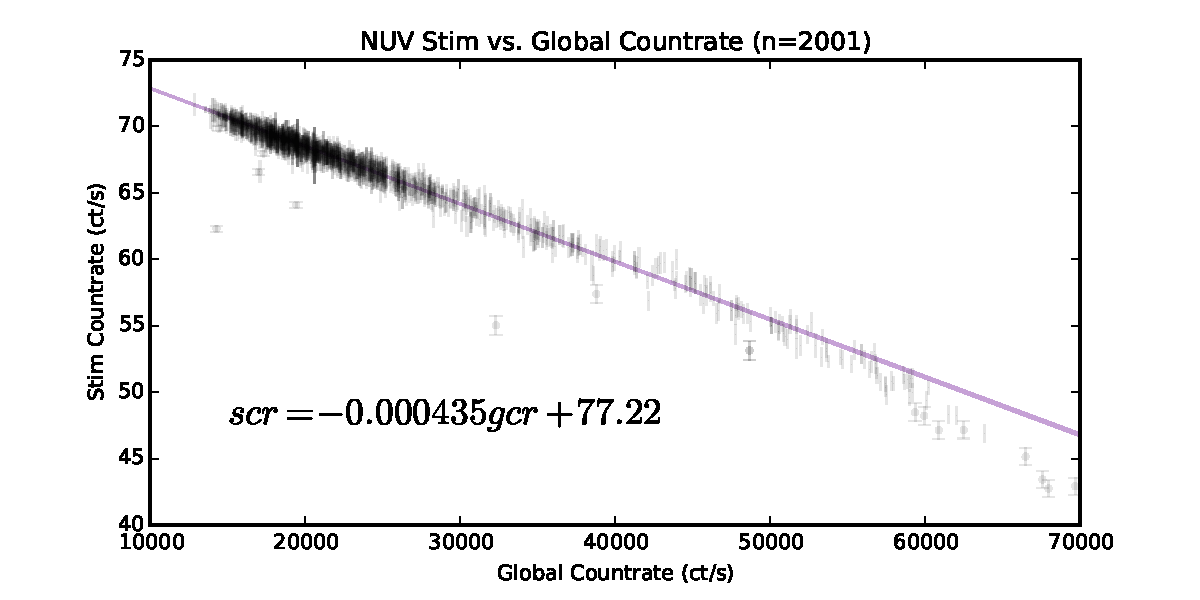
\includegraphics[scale=0.45]{Stim_v_GCR_NUV.pdf}
\caption{Over the course of a typical eclipse such as this one, the global count rate falls and then rises in a characteristic ``smiley face'' pattern due to light scattered by Earth's atmosphere. The scalloped, periodic variations throughout the eclipse are due to the dither pattern moving the spacecraft minutely, repeatedly toward and away from the Earth's limb during an eclipse.
\label{nuvstim}}
\end{figure}

\begin{figure}
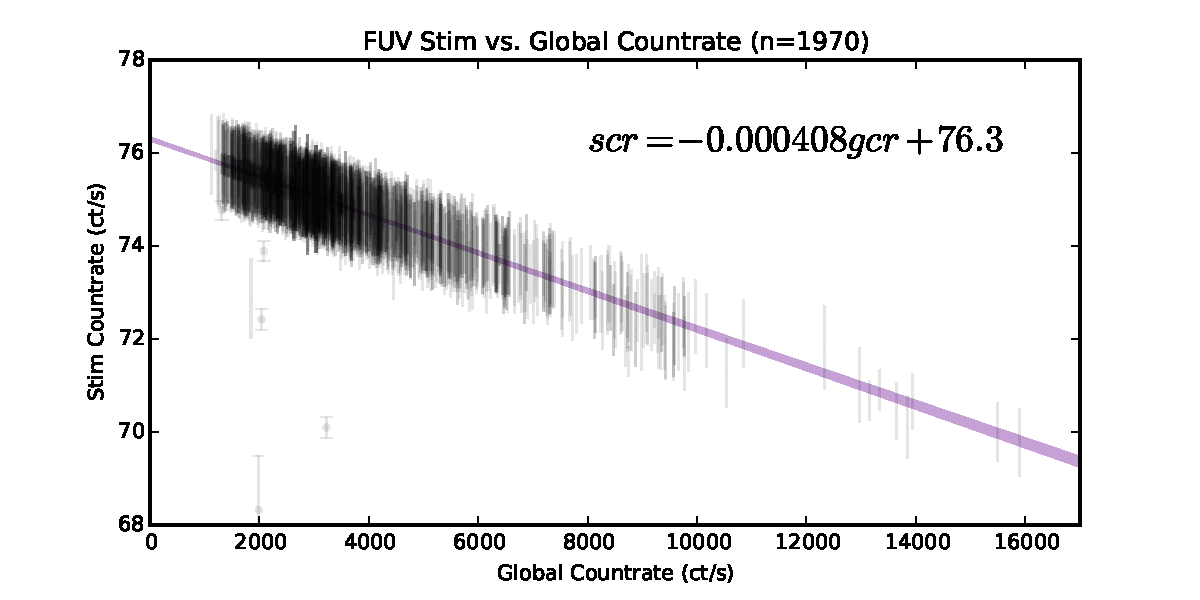
\includegraphics[scale=0.45]{Stim_v_GCR_FUV.pdf}
\caption{Over the course of a typical eclipse such as this one, the global count rate falls and then rises in a characteristic ``smiley face'' pattern due to light scattered by Earth's atmosphere. The scalloped, periodic variations throughout the eclipse are due to the dither pattern moving the spacecraft minutely, repeatedly toward and away from the Earth's limb during an eclipse.
\label{fuvstim}}
\end{figure}

In figures \ref{nuvstim} and \ref{fuvstim}, we plot global detector count rates against stim count rates with errors based on counting statistics. In calculating these rates, exposure times have corrected for shutter (see Section \ref{effexptime}), but not dead time. We fit a linear mixture model to the data, with both ``foreground'' and ``noise'' parameters. The model was sampled by Markov Chain Monte Carlo (MCMC) against the data for $\sim 2000$ observations in each band to produce maximum likelihood model parameters for the stim count rate as functions of global count rates, which can be converted to a fractional dead time by comparing the stim count rate against the reference rate. Rather than directly adopting the quoted stim reference rate of 79 cps for both bands, we used the maximum likely y-intercept value corresponding to ``zero'' global counts per second. At 77.2 and 76.3 cps in NUV and FUV respectively, the "nominal" stim rates, as measured, differ by 1.2\% from each other and 2.3\% and 3.5\% from the \emph{commanded} rate of 79 cps. The analysis suggests slopes that differ in each band by about 6.5\%. Less than $\sim 1\%$ of data in both bands were classified as noise. 

We interpret the apparently non-linear rolloff in NUV data at $\sim 50,000$ global cps to be a real effect, attributable to global detector gain sag as described in \citep{mor2007}. The linear empirical deadtime correction will therefore overestimate effective exposure times for very bright fields (where gAperture will produce erroneously dim flux estimates).

Note that the ratio of effective exposure time to raw exposure time is not constant over \emph{any} finite period. The detector FOV is constantly moving in relationship to the sky, creating small changes in field brightness and therefore global count rate. At the same time, the spacecraft is traveling through the shadow of the Earth and encountering shifts in ambient brightness due to airglow which, likewise, manifest as changes in global count rate. Researchers interested in the variability of targets within single observations should re-compute the exposure time for every bin in order to account for this effect. gAperture makes this correction automatically when creating a light curve.

\subsection{Relative Response Correction}
In the mission pipeline, variable sensitivity ("response") across the detector was corrected for by the application of relative response maps. These relative response maps (-rrhr) were composed of successive projections of an upsampled detector flat on the sky in one-second increments, weighted for effective exposure time over those increments. The response maps could then be divided out of the integrated count maps over the same time range to produce fully calibrated intensity maps (-int). In developing gPhoton, we discovered that not only did this repeated interpolation unnecessarily degrade the information in the flat, but it was also computationally intensive and slow. For this reason, we apply the flat at the detector level by weighting each individual photon event by the value of the pixel in the uninterpolated flat that corresponds to the detector location at which the event was recorded. The exposure time correction is applied as an independent separate step.

\subsection{Flux Uncertainties}
\label{fluxuncert}
The flux uncertainties produced by gAperture are computed by adding the counting errors in the aperture and background annulus in quadrature, as scaled to the area of the aperture. If there are relatively bright sources located in either the aperture or background annulus, then this underestimates total uncertainty in proportion to the brightness of the contaminating sources. Before relying on the estimated flux uncertainties, users are encouraged to visually check a full depth coadd of the targeted region (as created by gMap) for such sources. Future work will include thorough modeling of the imaging chain that allows for more accurate uncertainty propagation.

\subsection{Client vs. Server Optimizations}
\label{speedopt}
Early design concepts anticipated that a large amount of data processing would be offloaded to the database and server. In practice, we found that it was more convenient for both developers and users to conduct the majority of processing on the \emph{client}, and reserve server-side operations to standard SQL actions like merging columns or counting rows. In early builds of the gPhoton tools, we were also surprised to learn that the total client-side runtime was not dominated by processing time on either the client or server, but by the handling of the http requests themselves---that is, the time required just to send and receive a response from the server. As a result, runtimes were longer than we found acceptable. Significant development work has therefore gone into minimizing this issue. Among the most substantial and surprisingly effective strategies to minimizing requests has been to download almost \emph{all relevant data} to the client---anything within the targeted sky regions and time ranges, which can easily be millions of database rows---to the client early in each run, and performing most subsequent analysis on those data locally. (Some operations are still best performed on the server, such as counting the number of global counts in a time range for the purpose of computing a deadtime correction.) This reduces runtime dramatically, but also requires that the server pass very large volumes of data during gAperture or gMap, with the load made that much greater if there are multiple simultaneous users or one users performing multiple simultaneous runs. The upshot is that the needs of the gPhoton project are driving the server requirements for the entire MAST archive.

\section{Example Science Application - Stellar Flares From CR Draconis}
\label{scienceexamples}
CR Draconis (HIP 79796) is a fairly bright ($V \sim 10$) binary star system composed of two M dwarfs located $\sim 20$ pc away in a slightly eccentric orbit with a period of $\sim 4$ years \citep{tam2008}, and has been known to exhibit flares for many decades now \citep{cri1970}. The system was identified as a high-amplitude variable in the second version of the GALEX Ultraviolet Variability (GUVV-2) Catalog \citep{whe2008}, where a maximum NUV flux difference of two magnitudes was identified within the available visits at that time. \citet{wel2006} studied one CR Draconis' flare events with high temporal sampling by extracting light curves from sky-projected, ``extended'' (-x) photon list files, produced as non-standard products of the GALEX mission pipeline.

Using our gPhoton pipeline, we have searched for flares from the CR Dra system using all available GALEX data. The largest observed flare in GALEX is the one reported in \citet{wel2006}, but we also see seven additional flares, spanning from 2003 through 2011 (nearly 2 full orbits of the binary). Fig. \ref{crdraflares} shows each of the identified flares. When available, the FUV version of the light curves are shown in blue.  Several of the flares are double-peaked, and some show elevated levels of flux before or after the flare event.  There is also a range of amplitudes and durations, with some increasing in flux by less than a factor of two and lasting only a few minutes in duration. These short-duration flares have less an energy than the longer duration, stronger flares, but also can occur more frequently, and thus may still impact the habitability of exoplanets in those systems \citep[e.g.,][]{ram2013}. While the total energy in a given flare event would be lower, there is also an increased chance for flare-planet alignment. There have also been studies of the flare rates in resolved M dwarf binaries as a function of orbital separation. The number of such binaries is small, but CR Draconis is one candidate, and given that the GALEX time baseline extends two full orbital periods, could improve the statistics from previous studies \citep{tam2008}.  {\color{red}Is the difference in flare times for FUV and NUV real, or a bug in the code, or an effect of using $t_{\rm{mean}}$ that may result in different time stamps per point.  Should only differ by a few seconds though, so seems unlikely it would show up that clearly.}

\begin{figure}
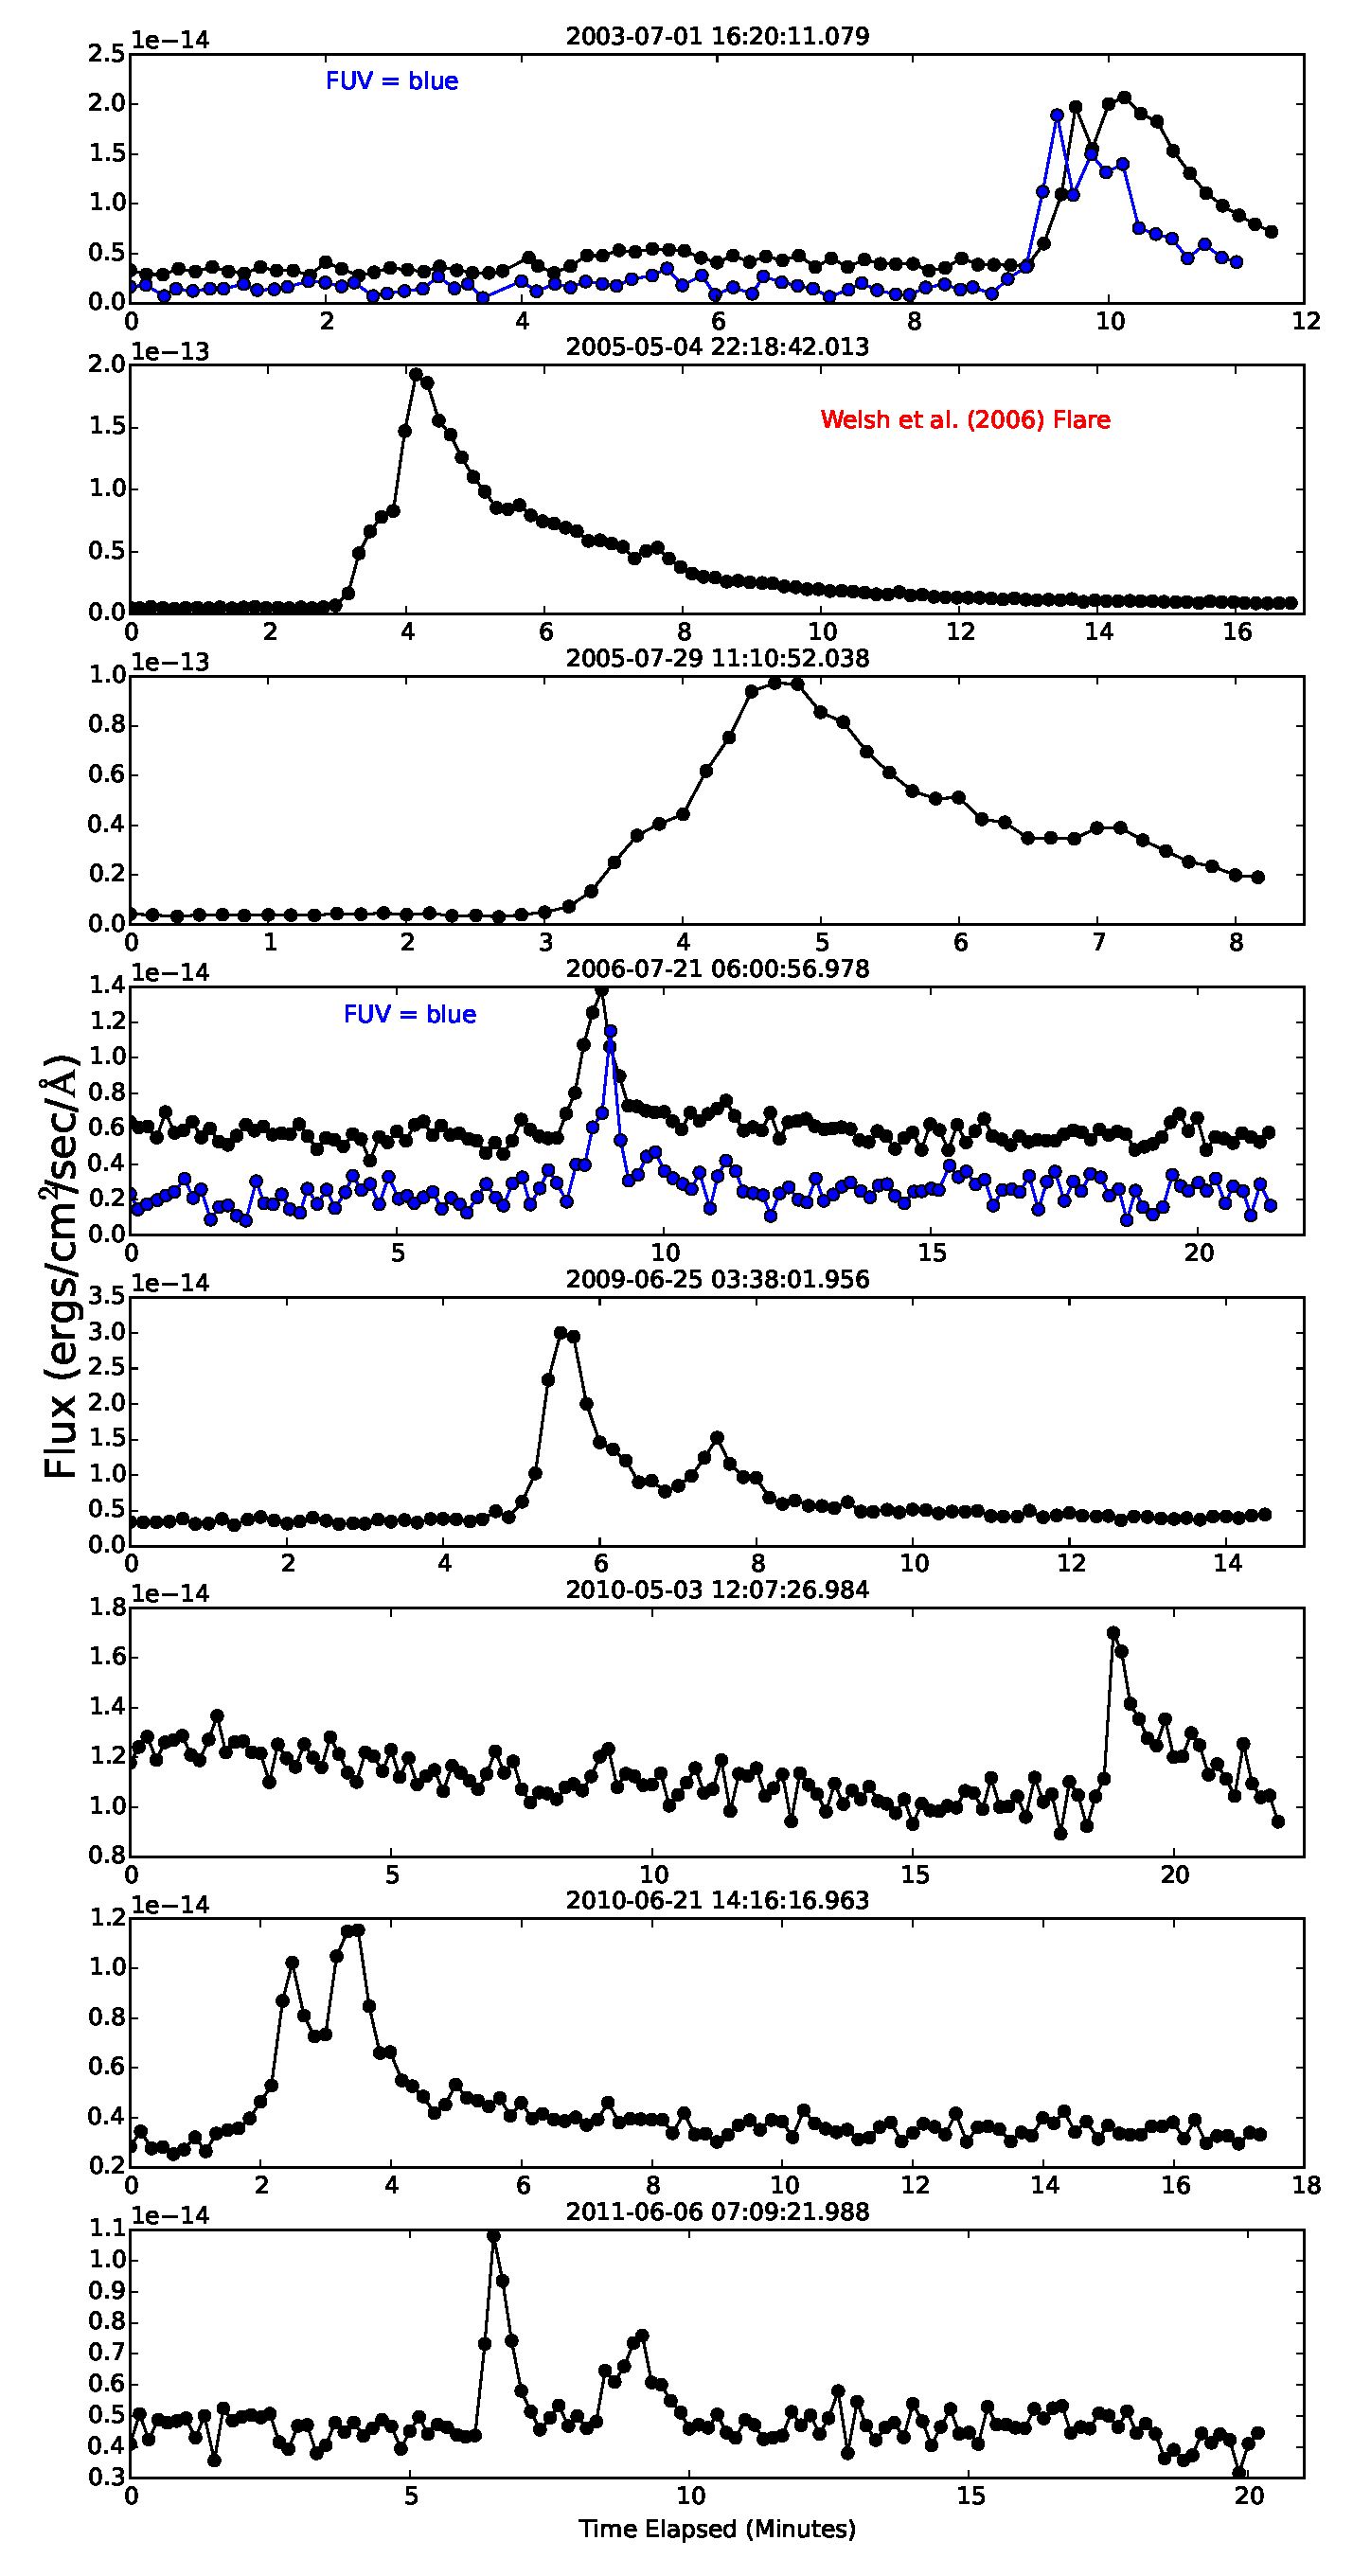
\includegraphics[scale=0.375]{FigCRDraFlares.eps}
\caption{Flares detected on CR Draconis using gPhoton, across the lifetime of the mission.  When available, FUV light curves are plotted (in blue) along with the NUV curves (in black).  Fluxes have not been aperture corrected. \label{crdraflares}}
\end{figure}

A detailed analysis of the flares is beyond the scope of this introductory paper, which serves to present the software itself, and is reserved for future papers that will focus on the astrophysics of flare stars with gPhoton.  However, it is instructive to provide some short scripts demonstrating the basic work flow when creating the plot shown here.  To define our photometric aperture, we used gMap to construct a deep coadd image, centered on CR Draconis, using all available photon events (Fig. \ref{crdracoadd}). Here's the example script that was used, which assumes you have installed gPhoton such that the software lies in your PYTHONPATH environment variable, and thus can be imported as a package (see Inline Supplementary Code \#1, available in the online version of the article):

%InlineCodeSupplementary01.txt gets placed here in the online version of the article.

With our apertures defined (we also adjusted the center of the apertures, due to the moderate proper motion of the star), we can construct our light curve file using gAperture. Here's the example script that was used to create the CSV file (see Inline Supplementary Code \#2, available in the online version of the article):

%InlineCodeSupplementary02.txt gets placed here in the online version of the article.

After the CSV file is created, we wrote a separate script that reads in the CSV file, converts the $t_{\rm{mean}}$ timestamps from GALEX time to Julian Date, and then defined x-axis boundaries to center on each of the eight flare events of interest. Note that we did not apply aperture corrections to the fluxes shown in Fig. \ref{crdraflares}, but such corrections are available in Fig.\ 4 in \citet{mor2007}.  A simple interpolation scheme is provided in gPhoton, using those values, called ``apcorrect1'' within the ``galextools.py'' module.

\begin{figure}
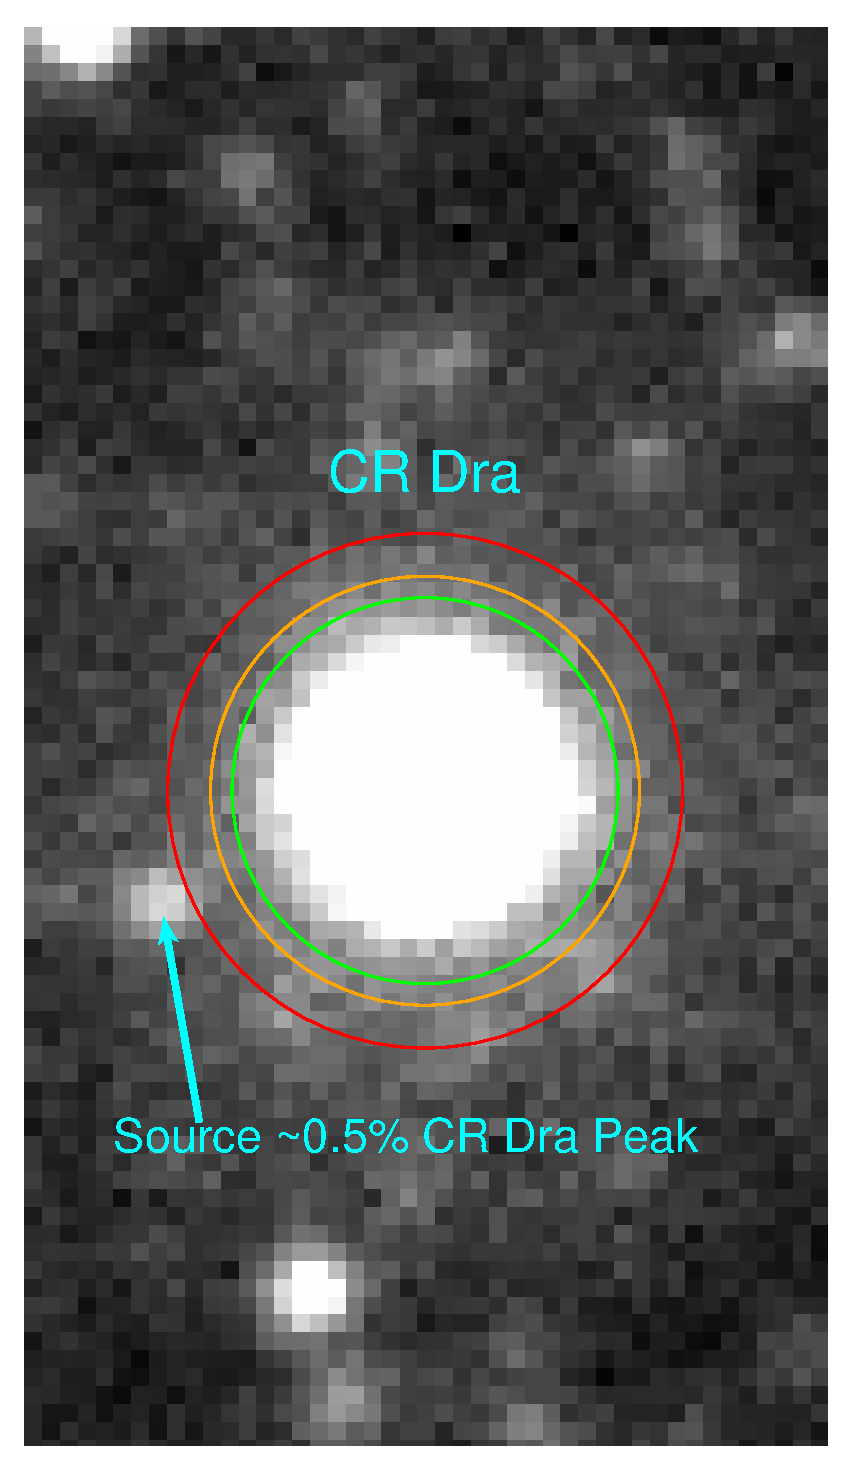
\includegraphics[scale=0.375]{FigCRDraCoadd.eps}
\caption{Deep coadd image of CR Draconis using all available NUV photon events. The image is in counts, since we are only looking to define our photometric aperture and search for possible contamination sources. The aperture, inner annulus, and outer annulus for photometry are represented by the green, orange, and red circles, respectively.  There is a source to the lower left that is $\sim 0.5$\% the peak of CR Draconis itself. Although testing showed it did not have a major impact on the photometry significantly, we still define our apertures such that it is not included within them.\label{crdracoadd}}
\end{figure}

\section{Conclusion}
The GALEX mission was extremely productive and is likely among the most influential ultraviolet astronomical surveys for the foreseeable future. The gPhoton project extends the utility of this data set well beyond the scientific objectives of the original mission, most specifically towards the study of short time domain UV variability.

Some of the techniques developed for gPhoton can be applied to other data sets produced by non-integrating detectors, particularly micro-channel plates. The fact that spatial analyses can be performed by making direct queries at the photon-level data, rather than artificially degrading the spatial resolution of the data by integrating and interpolating into pixelated images, offers potential advantages in terms of both the flexibility of the data archive and the computational overhead for some types of analysis. The corresponding data management and volume issues associated with storing and retrieving massive amounts of photon-level data is not trivial, but also entirely solvable with appropriate use of existing, off-the-shelf database and storage technology.

The gPhoton project is also a trial in a new paradigm for data archiving, where the functioning machinery for generating higher level data from lower---the calibration pipeline---is incorporated into the data archive itself. Even when preparation of the higher level data for archiving is well documented and comprehensible to future researchers, the priorities, interests, and needs of those users may not be the same as the data creators or archivists. At present, the standard recourse in such cases is to go back to some minimally reduced version of the data and create a new tools or procedures for reducing the data from scratch. This can be onerous, time consuming, or impossible depending on the type of data, the quality of the documentation, and the availability of members of the original project team to answer inevitable questions. Especially when the data record observations that are unique or would be difficult to reproduce---for example, of rare astrophysical events in wavelengths only detectable above the atmosphere---an inability to reanalyze the data represents a true loss for research. Incorporating a \emph{functioning} calibration pipeline into the archive significantly lowers the barrier for future researchers to modify that machinery to produce new science that was not anticipated by the original project teams.

The behavior of the GALEX detector during very short timespans (which correspond to small spatial sampling of the detector) is not well characterized, and further work on improving the resolution of the detector flat fields, as well as correctly propagating flux uncertainties, will be required to derive the maximum utility from the photon-level data.

\section{Acknowledgments}
{\color{red}Place acknowledgments here, waiting to here back from Rick White about this.  Also need to add, at least, MAST acknowledgment, GALEX one, Simbad one.  Anything else?} We thank the GALEX beta testers for their feedback and patience, particularly Raghvendra Sahai (JPL), William Adler (JPL), {\color{red}Clare ??? (???)}, and {\color{red}NYU people}. We also thank several former members of the GALEX mission team at Caltech for providing access to and consultation on the mission data, software, and calibration, including Patrick Morrissey, Don Neill, Min Hubbard, Tim Conrow, Ted Wyder, and Karl Forster.

\bibliography{gphoton}

\end{document}
